% !TEX program = lualatex
% Working paper version of the thesis. Tables and figures are \input from
% Tables_and_Figures/, which Syntax/0_master.do regenerates. Everything cut from
% this version lives in online_appendix.tex.
\documentclass[12pt]{article}
% Shared preamble for paper.tex and online_appendix.tex
% Standard economics working-paper layout: 12pt, 1-inch margins, 1.5 spacing,
% author-year citations. Compile with LuaLaTeX.

\usepackage[margin=1in]{geometry}
\usepackage{setspace}
\onehalfspacing
\usepackage{amsmath, amssymb}
\usepackage{graphicx}
\graphicspath{{Tables_and_Figures/figures/}{static_figures/}}
\usepackage{booktabs, tabularx, threeparttable, array, makecell, longtable}
\usepackage{ragged2e}
\usepackage{placeins}
\usepackage{xcolor}
\usepackage[bottom]{footmisc}
\usepackage[font=small, labelfont=bf]{caption}
\usepackage{enumitem}
\setlist{itemsep=2pt, topsep=4pt}

% Author-year citations, as in most economics working papers
\usepackage[backend=biber, style=authoryear, natbib=true, maxcitenames=2,
  uniquename=false, uniquelist=false, giveninits=true, dashed=false]{biblatex}
\addbibresource{articles.bib}
% Undated web sources show "n.d." instead of the year they were accessed
\DeclareLabeldate{\field{date}\field{year}\field{eventdate}\field{origdate}\literal{nodate}}
% Let long URLs in the references break across lines
\usepackage{xurl}
\setcounter{biburllcpenalty}{7000}
\setcounter{biburlucpenalty}{8000}
\setcounter{biburlnumpenalty}{9000}

% Web links are blue and clickable; internal references and citations stay
% black but are still clickable. URLs use the same font as the text.
\usepackage[colorlinks=true, urlcolor=blue, filecolor=blue, linkcolor=black, citecolor=black]{hyperref}
\urlstyle{same}
\newcommand{\appendixurl}{https://github.com/calvinpan1/thesis_india_diaspora_engagement_policies/blob/main/online_appendix.pdf}
\newcommand{\repourl}{https://github.com/calvinpan1/thesis_india_diaspora_engagement_policies}

% Column types and helpers used by the generated tables
\newcolumntype{L}[1]{>{\RaggedRight\arraybackslash}p{#1}}
\newcolumntype{Y}{>{\RaggedRight\arraybackslash}X}
\newcolumntype{Z}{>{\Centering\arraybackslash}X}
\newcolumntype{C}[1]{>{\Centering\arraybackslash}p{#1}}
\renewcommand{\arraystretch}{1.2}
\setlength{\emergencystretch}{2em}
\setlength{\LTcapwidth}{\textwidth}
\newcommand{\fulltablenote}[2]{%
  \multicolumn{#1}{@{}>{\RaggedRight\arraybackslash}p{\dimexpr\linewidth-2\tabcolsep\relax}@{}}{\footnotesize #2}\\%
}

% Tables and figures read single-spaced
\AtBeginEnvironment{table}{\singlespacing}
\AtBeginEnvironment{figure}{\singlespacing}
\AtBeginEnvironment{longtable}{\singlespacing}


% Cross-references to the online appendix (see crossrefs.tex)
% Generated by make_crossrefs.py -- do not edit by hand.
% \oaref{label}: number of a section, table, or figure in the online appendix.
% \pref{label}:  number of a section, table, or figure in the paper.
\newcommand{\oaref}[1]{\ifcsname oaref@#1\endcsname\csname oaref@#1\endcsname\else\textbf{??}\fi}
\newcommand{\pref}[1]{\ifcsname pref@#1\endcsname\csname pref@#1\endcsname\else\textbf{??}\fi}
\expandafter\def\csname oaref@FDI threats\endcsname{4.1.2}
\expandafter\def\csname oaref@fig:Non-Econ vs Econ\endcsname{A15}
\expandafter\def\csname oaref@fig:admin_unit_creation_date\endcsname{A19}
\expandafter\def\csname oaref@fig:all companies by sector\endcsname{A22}
\expandafter\def\csname oaref@fig:bengali speakers\endcsname{A5}
\expandafter\def\csname oaref@fig:commercialcount\endcsname{A11}
\expandafter\def\csname oaref@fig:dravidian_languages\endcsname{A2}
\expandafter\def\csname oaref@fig:econ DEP types over time\endcsname{A20}
\expandafter\def\csname oaref@fig:econ DEPs by state\endcsname{A17}
\expandafter\def\csname oaref@fig:fditop50_noindialine\endcsname{A7}
\expandafter\def\csname oaref@fig:fdivalue\endcsname{A8}
\expandafter\def\csname oaref@fig:ictcount\endcsname{A10}
\expandafter\def\csname oaref@fig:indo_aryan_key\endcsname{A1}
\expandafter\def\csname oaref@fig:info_timing\endcsname{A21}
\expandafter\def\csname oaref@fig:jaccard\endcsname{A18}
\expandafter\def\csname oaref@fig:jobs\endcsname{A9}
\expandafter\def\csname oaref@fig:nepali speakers\endcsname{A6}
\expandafter\def\csname oaref@fig:non-econ DEPs by state\endcsname{A16}
\expandafter\def\csname oaref@fig:punjabisovertime\endcsname{A3}
\expandafter\def\csname oaref@fig:sample 3\endcsname{A14}
\expandafter\def\csname oaref@fig:sample1\endcsname{A13}
\expandafter\def\csname oaref@fig:sample1 gujarati diaspora\endcsname{A12}
\expandafter\def\csname oaref@fig:tamil speakers\endcsname{A4}
\expandafter\def\csname oaref@sec:oa_deps\endcsname{5}
\expandafter\def\csname oaref@sec:oa_discussion\endcsname{8}
\expandafter\def\csname oaref@sec:oa_identification\endcsname{6}
\expandafter\def\csname oaref@sec:oa_measurement\endcsname{4}
\expandafter\def\csname oaref@sec:oa_replication\endcsname{1}
\expandafter\def\csname oaref@sec:oa_results\endcsname{7}
\expandafter\def\csname oaref@sec:oa_roadmap\endcsname{2}
\expandafter\def\csname oaref@sec:oa_states\endcsname{3}
\expandafter\def\csname oaref@sec:oa_techhubs\endcsname{9}
\expandafter\def\csname oaref@ss: bundled, rare policies\endcsname{6.4}
\expandafter\def\csname oaref@ss: model mechanics\endcsname{6.5}
\expandafter\def\csname oaref@ss: sector\endcsname{7.1}
\expandafter\def\csname oaref@ss:activity\endcsname{7.2}
\expandafter\def\csname oaref@ss:are there deps\endcsname{3.2}
\expandafter\def\csname oaref@ss:comp size\endcsname{7.3}
\expandafter\def\csname oaref@ss:diaspora description\endcsname{4.2.4}
\expandafter\def\csname oaref@ss:diaspora languages, state selection\endcsname{3.1}
\expandafter\def\csname oaref@ss:diaspora_measurement_strategy\endcsname{4.2.1}
\expandafter\def\csname oaref@ss:endogeneity\endcsname{6.8}
\expandafter\def\csname oaref@ss:expectations\endcsname{6.9}
\expandafter\def\csname oaref@ss:ict\endcsname{7.4}
\expandafter\def\csname oaref@ss:logical threats\endcsname{6.6}
\expandafter\def\csname oaref@ss:operationalizing DEPs\endcsname{5.2}
\expandafter\def\csname oaref@ss:operationalizing FDI\endcsname{4.1}
\expandafter\def\csname oaref@ss:operationalizing diasporas\endcsname{4.2}
\expandafter\def\csname oaref@ss:reliability\endcsname{4.2.3}
\expandafter\def\csname oaref@ss:samples\endcsname{4.2.2}
\expandafter\def\csname oaref@ss:source_country_roadmap\endcsname{2.1}
\expandafter\def\csname oaref@ss:specification\endcsname{6.2}
\expandafter\def\csname oaref@ss:spillovers\endcsname{6.7}
\expandafter\def\csname oaref@ss:why the us?\endcsname{2.2}
\expandafter\def\csname oaref@ss:why_ppml\endcsname{6.1}
\expandafter\def\csname oaref@subsection:DEPs descriptives\endcsname{5.2.1}
\expandafter\def\csname oaref@subsection:FDI descriptives\endcsname{4.1.3}
\expandafter\def\csname oaref@subsection:no operationalizing DDI\endcsname{4.1.1}
\expandafter\def\csname oaref@tab:appendix_singlepolicy\endcsname{A25}
\expandafter\def\csname oaref@tab:dep_turnon_events\endcsname{A7}
\expandafter\def\csname oaref@tab:final_activity_appendix_singlepolicy\endcsname{A12}
\expandafter\def\csname oaref@tab:final_activity_table2_h1\endcsname{A10}
\expandafter\def\csname oaref@tab:final_activity_table4_h3\endcsname{A11}
\expandafter\def\csname oaref@tab:final_cluster_appendix_singlepolicy\endcsname{A9}
\expandafter\def\csname oaref@tab:final_cluster_table4_h3\endcsname{A8}
\expandafter\def\csname oaref@tab:final_company_size_h0\endcsname{A13}
\expandafter\def\csname oaref@tab:final_company_size_table1_baseline\endcsname{A14}
\expandafter\def\csname oaref@tab:final_company_size_table3_h2\endcsname{A15}
\expandafter\def\csname oaref@tab:final_ict_company_size_appendix_singlepolicy\endcsname{A22}
\expandafter\def\csname oaref@tab:final_ict_company_size_table2_h1\endcsname{A20}
\expandafter\def\csname oaref@tab:final_ict_company_size_table4_h3\endcsname{A21}
\expandafter\def\csname oaref@tab:final_ict_company_size_techhubs_table2_h1\endcsname{A23}
\expandafter\def\csname oaref@tab:final_ict_company_size_techhubs_table4_h3\endcsname{A24}
\expandafter\def\csname oaref@tab:final_ict_generations_education_appendix_singlepolicy\endcsname{A17}
\expandafter\def\csname oaref@tab:final_ict_generations_education_table4_h3\endcsname{A16}
\expandafter\def\csname oaref@tab:final_ict_worker_appendix_singlepolicy\endcsname{A19}
\expandafter\def\csname oaref@tab:final_ict_worker_table2_h1\endcsname{A18}
\expandafter\def\csname oaref@tab:jaccard_top10\endcsname{A6}
\expandafter\def\csname oaref@tab:language_fdi_a1\endcsname{A2}
\expandafter\def\csname oaref@tab:language_fdi_a2\endcsname{A3}
\expandafter\def\csname oaref@tab:language_fdi_a3\endcsname{A4}
\expandafter\def\csname oaref@tab:language_fdi_a4\endcsname{A5}
\expandafter\def\csname oaref@tab:language_fdi_sample\endcsname{A1}
\expandafter\def\csname oaref@tab:single_firm_tech_localities\endcsname{A26}


\title{Do Subnational Diaspora Engagement Policies Attract FDI?\\ Evidence from India}
\author{Calvin Pan\thanks{University of Virginia, Batten School of Public Policy. This paper is based on my undergraduate thesis in the Distinguished Majors Program in Foreign Affairs. An \href{\appendixurl}{online appendix} and a \href{\repourl}{replication package} accompany the paper.}}
\date{October 2026}

\begin{document}
\maketitle
\thispagestyle{empty}

\begin{abstract}
\noindent Many federal, multi-ethnic countries, such as India, have subnational units (states and provinces) that correspond closely to particular ethnic or linguistic communities, and many of those units have adopted their own diaspora engagement policies (DEPs). Yet the diaspora literature rarely examines these policies, and the FDI literature rarely treats subnational diasporas as a factor in firm location choice. This paper provides the first empirical study of subnational DEPs' effectiveness in attracting foreign direct investment (FDI). Using an original dataset of 44 DEPs across 8 Indian states from 2005--2017, I generate Poisson pseudo-maximum likelihood (PPML) gravity estimates of how DEPs moderate the influence of subnational diasporas in individual US metro areas on FDI inflows to their home states. I find, first, that Indian state diasporas in US metros have a significant association with FDI inflows to their home states, while the Indian national diaspora does not. Second, subnational DEPs matter most clearly for Information and Communications Technology (ICT) FDI, not for all FDI: if a subnational diaspora doubles in a city, a state that adopts \textit{any} DEP is associated with about 15\% more ICT FDI projects from that city than it would receive without one. Third, investment-facing informational DEPs are the most consistently positive. Subnational DEPs can attract FDI, but only when they reduce concrete transaction costs for diaspora investors in sectors where diaspora members possess real informational and network advantages.

\vspace{1em}
\noindent \textbf{JEL codes:} F21, F22, F23, H77, O53\\
\noindent \textbf{Keywords:} diaspora engagement policies, diaspora direct investment, foreign direct investment, subnational governments, India, PPML gravity
\end{abstract}

\newpage
\setcounter{page}{1}

%==============================================================================
\section{Introduction} \label{sec:intro}
%==============================================================================

On an average day in Thiruvananthapuram in the Indian state of Kerala, the seven-story tower of the Department of Non-Resident Keralites Affairs (NORKA Roots) bustles with activity. On the third floor, the Pravasi Welfare Board funds education grants, pensions, health insurance, and even weddings for its 930 thousand registered members. On the fourth floor, where the head office is, diaspora businessmen negotiate favorable loan terms with bureaucrats, planning out their next big investment back home. On the sixth and seventh floors, the Non-Resident Indian (NRI) Commission mediates grievances and issues rulings with all the powers of a civil court. For the 8 million Keralites who live outside of Kerala -- 20\% of all Keralites in the world -- NORKA Roots serves as an indispensable lifeline.

This story is repeated across India: Gujarat, Punjab, Tamil Nadu, and other states all maintain their own relationships with their own diasporas. It also has echoes around the world. Many federal and multi-ethnic countries have states, provinces, republics, or regions that court overseas populations through diaspora ministries, investment roadshows, grievance mechanisms, origin cards, matching-fund programs, and business facilitation schemes. In some cases, these subnational diaspora engagement policies (DEPs) appear to do more direct work than national institutions: a Punjabi investor trying to recover land, a Malayali return migrant seeking a loan, or a Gujarati entrepreneur looking for tax guidance often needs a state-level institution, not just a national ministry.

Yet the diaspora literature rarely examines these subnational policies, preferring to remain at the national level \citep{gazzotti_embracing_2023}. This is costly because diasporas are not always national in practice. In multi-ethnic countries, migrants often maintain attachments to a region, language, province, city, or hometown that is more precise than the nation-state. A Telugu-speaking investor in Dallas may not simply be an ``Indian'' investor; she may have information, networks, and preferences that make investment in Andhra Pradesh or Telangana more plausible than investment in Punjab or Kerala.

The FDI literature also has reason to care. Many subnational DEPs are designed to attract cross-border financial flows, especially foreign direct investment (FDI), or investment in which an investor in a sending country controls more than 10\% of an asset in a recipient country. FDI scholars have long studied why firms choose one country over another, and diaspora scholars have shown that migrants can facilitate investment into their countries of origin. But very little work asks whether governments can amplify that diaspora effect through policy, and no study has yet examined whether subnational DEPs affect diaspora-influenced FDI.

This gap exists because the question is hard to study. It requires subnational DEP data, subnational diaspora measurement in a sending country, and subnational FDI destinations in a recipient country. Most settings do not provide all three. Even when they do, identification is difficult because states that adopt DEPs may differ systematically from states that do not. This paper addresses those barriers by studying India, where state-language mappings, US Census/ACS language data, project-level FDI data, and staggered state-level DEP adoption make a quantitative analysis possible.

Using an original dataset of 44 DEPs across 8 Indian states from 2005--2017, I generate Poisson pseudo-maximum likelihood (PPML) gravity estimates of how DEPs moderate the influence of subnational diasporas in individual US metro areas on FDI inflows to their home states. This design contributes four innovations. First, I build an original state-year dataset of Indian subnational DEPs. Second, I measure subnational diasporas using US Census/ACS language data. Third, I disaggregate the US diaspora into metro areas, allowing comparisons across high- and low-diaspora metro-state dyads. Fourth, I use project-level greenfield FDI data, which allows me to study sector-specific FDI rather than pooling all investment together.

I first find that Indian state diasporas in US metros have a significant association with FDI inflows to their home states, while the Indian national diaspora does not. I then find that at both the extensive and intensive margins, subnational DEPs matter most clearly for tech FDI. If a subnational diaspora doubles in population in a city, an Indian state that adopts \textit{any} DEP is associated with 15\% more Information and Communications Technology (ICT) FDI projects from that city than it would receive without one. I then decompose DEPs into policy types and find that the strongest evidence comes from investment-facing informational policies, especially policies that reduce tax, regulatory, bureaucratic, and information barriers. The ICT result survives among small companies, holds across several definitions of the diaspora, and points toward educated founders, managers, and investors rather than current tech workers as the people DEPs reach.

These results change our understanding of both diaspora engagement and FDI. For the diaspora literature, they show that subnational governance is not merely symbolic or descriptive. For the FDI literature, they show that diasporas matter not just as national migrant stocks, but as subnational networks that can influence firm location choice within a country. For policymakers, they show that diaspora-specific policies add value only when they solve diaspora-specific problems. A generic investment promotion agency can advertise opportunities to everyone. A diaspora-specific DEP matters when it helps nonresident investors navigate legal status, repatriation rules, property disputes, local bureaucracies, trustworthy partners, and state-specific investment procedures.

The policy implication is therefore conditional rather than universal. Subnational DEPs can be worth investing in, but governments that want diaspora FDI must adopt policies that are seriously investment-focused. Welfare, cultural, grievance, or rural-development DEPs may serve important purposes, but they are unlikely to attract investment on their own. The ICT specificity of these results should also be generalized cautiously: India is an unusually high-FDI country with an unusually important ICT sector. The broader lesson is that governments should identify the sectors where their diaspora has real information, trust, and decision-making advantages, then design DEPs around those barriers.

The rest of the paper proceeds as follows. Section~\ref{sec:lit} reviews the literature on diaspora direct investment and DEPs and lays out the hypotheses. Section~\ref{sec:setting} explains why India and the United States make a workable case. Section~\ref{sec:data} describes the data, Section~\ref{sec:strategy} the empirical strategy, and Section~\ref{sec:results} the results. Section~\ref{sec:discussion} discusses what the results mean for policy, and Section~\ref{sec:conclusion} concludes. The online appendix contains the full case-selection roadmap, measurement details, the DEP codebook and descriptives, and an extended identification discussion. Online Appendix Section~\oaref{sec:oa_results} reports the robustness checks: the main results across alternative diaspora definitions (generation, education, ICT occupation), by company size, in tech-hub metros only, by sector and project activity, and single-policy estimates for every DEP grouped by how many states and years adopt it.

%==============================================================================
\section{Literature and Theory} \label{sec:lit}
%==============================================================================

\subsection{Diaspora direct investment}

There is a well-documented link between diasporas and FDI. \citet{leblang_familiarity_2010} finds in an examination of 56 FDI-source countries and 154 FDI-destination countries that there is a ``migration elasticity'' of 0.2: for every 1\% increase in the migrant stock in the source country, there is a 0.2\% increase in FDI to the destination country. Other papers replicate this finding for similar populations: refugees and immigrants to the US across 130 years \citep{mayda_refugees_2022, burchardi_migrants_2019}.

Is this merely a correlation, or is there something systematically different about diaspora investors that make them invest more in their home countries? Current literature postulates that diaspora investors are different in three ways. First, they have an informational advantage. Their network tells them about opportunities that others do not know about, and their lived experiences allow them to more accurately assess the prospects of an opportunity \citep{leblang_familiarity_2010, useche_highly_2020}. \citet{kugler_migration_2018} confirm this by finding that the positive effect of diasporas on investment is magnified for culturally distant destination countries where non-diaspora investors have less information. Second, diasporas simply prefer home. \citet{nielsen_investing_2009} theorize that diaspora members' investment decisions may be influenced by non-financial reasons like social status and emotional gain, or ``warm glow'' \citep{andreoni_impure_1990}. Finally, companies that hire diaspora members become more familiar with those diaspora members' home countries. As \citet{kapur_diasporas_2001} puts it, ``Companies like Yahoo, Hewlett Packard and General Electric have opened R\&D centers in India largely because of the confidence engendered by the presence of many Indians working in their US operations.''

In addition to making location decisions differently, diaspora members also run their firms differently. \citet{boly_diaspora_2014} examine diaspora investments across 19 different Sub-Saharan African countries and find that diaspora firms have better export performance and labor productivity compared to domestic firms. \citet{liu_under_2019} also show that returning diaspora Chinese entrepreneurs' overseas business knowledge makes their firms perform better.

These clear differences between how diaspora- and non-diaspora-influenced firms behave have led scholars to treat diaspora investment as a distinct subfield of FDI under the name Diaspora Direct Investment (DDI). Coined by a 2009 USAID report \citep{debass_diaspora_2009}, the term has become widespread enough to warrant a special issue on it \citep{alam_iqbal_introduction_2024}. DDI is not just about diaspora CEOs of large multinationals. Rather, it encompasses diaspora members who influence investment decisions at every level of the corporate hierarchy and even those outside the company entirely. The entire C-suite matters \citep{coda_zabetta_foreign-origin_2025}, diaspora entrepreneurs leading smaller firms have the same effect \citep{inouye_counteracting_2020}, and even non-controlling diaspora owners increase the likelihood of internationalization \citep{rabbiosi_diaspora_2019}. Because even non-employee diaspora members can influence FDI, the definition the field has converged on is the broader idea of the positive \textit{influence} all diaspora members can have on FDI to their home countries.

DDI is only one part of a larger set of financial flows that diaspora members facilitate between their host and home countries. Portfolio investment, bank loans, foreign exchange trading, and, of course, remittances form the remainder, and all of those have been heavily investigated by diaspora researchers. However, DDI is distinct from those flows because it is more intentional and permanent. As \citet{naujoks_transnational_2022} puts it, ``The motivation of the direct investor is a strategic long-term relationship with the direct investment enterprise to ensure a significant degree of influence by the investor in the management of the direct investment enterprise.''

DDI matters for FDI researchers as well, because it speaks to both of the main questions facing FDI research \citep{pandya_political_2016}. States may open to FDI not only because of general globalization pressure, but also because they seek to mobilize diaspora capital, skills, and political support. And when companies decide where to locate, DDI research introduces the diaspora as an important segment of decision-makers whose preferences we can study.

\subsection{Diaspora engagement policies and DDI}

DDI researchers have identified understanding how diaspora engagement policies (DEPs) affect DDI as a priority for the field. \citet{alam_iqbal_introduction_2024} identify how recipient country governments can best attract DDI as one of three major research areas, and \citet{naujoks_transnational_2022}'s research agenda calls on scholarship to ``address systematically whether and under what conditions specific policies have an effect on the volume, composition, and impact of inward diaspora investments.''

It is important to note that most DEPs are not explicitly economic. Many diaspora agencies are not designed with the main goal of attracting investment or have it as just one of their many goals \citep{gamlen_explaining_2021}. Some agencies, like the Philippines' Overseas Workers Welfare Administration, are designed around ensuring migrant welfare; others, like Mexico's Institute of Mexicans Abroad, are designed around fostering a sense of homeland connection \citep{orbeta_institutions_2009, delano_alonso_shifting_2018}. Based on those different goals, \citet{gamlen_human_2019} divides diaspora agencies and their DEPs into three types: those built to ``tap'' the diaspora for resources (e.g. taxation, investment schemes), those meant to ``embrace'' the diaspora (e.g. diaspora holidays), and those meant to ``govern'' the diaspora (e.g. overseas voting rights, resident cards). The ``tapping'' type has been studied most, and is generally subdivided into four categories: networks (e.g. a forum of high-net-worth investors), soft facilitation (e.g. matching diaspora members to projects), legal/regulatory advantages (e.g. opening up closed sectors for diaspora investors only), and hard economic advantages (e.g. lower loan terms or tax credits).

This distinction matters because diaspora-specific policies must provide something that general investment-promotion policies do not. A generic investment promotion agency can lower information costs for all investors. A diaspora-specific policy adds value only when it addresses the particular frictions that diaspora investors face or uses the particular advantages that diaspora investors possess. Diaspora investors often have local knowledge, language skills, family connections, and emotional attachment, but they may also face nonresident legal status, uncertainty about repatriation, property disputes, absentee ownership problems, and distrust of local bureaucracy. A DEP is therefore not just a smaller version of an investment promotion policy. It is potentially a tool for converting diaspora-specific knowledge and attachment into actual investment.

Even DEPs that are not explicitly economic may attract DDI by strengthening homeland preference. In the only quantitative test of DEPs' effect on DDI specifically, \citet{park_courting_2021} found in a study of 25 developing Asian states from 2002--2011 that ``psychological'' DEPs like hosting a diaspora forum and bestowing awards are the only statistically significant DEPs, while legal and informational DEPs do not raise DDI. However, only 10 DEPs were considered in that study, and its informational category contained just three policies, two of which might be better placed under psychological DEPs. A reexamination of variation in policy effects by category is warranted. Though not focusing on FDI, \citet{gamlen_human_2019} find that diaspora institutions double the effect of remittances on new business starts, which supports the idea that DEPs can amplify other cross-border financial flows.

This paper also suggests an important qualification: attachment alone may not be enough for FDI. Symbolic and welfare-oriented policies may build goodwill, but investment decisions also require credible information, procedural clarity, and expected returns. For diaspora members who already possess some emotional attachment, the binding constraint may not be whether they care about the homeland, but whether they can identify a credible project, navigate the local bureaucracy, understand their legal status, and resolve problems from abroad. This is especially true for FDI, which is more strategic and permanent than remittances or small-scale donations.

\subsection{A gap: subnational DEPs and DDI}

DDI scholars have identified subnational DEPs as an area where more research is urgently needed. \citet{naujoks_transnational_2022}'s research agenda states that ``beyond monolithic conceptualizations, analytical frameworks need to make meaningful differentiations that consider the heterogeneity of diaspora populations, the various economic sectors or subnational units.'' \citet{gevorkyan_diaspora_2022}'s systematic review notes that links between diasporas and home countries are often ``sector, event, or location specific.'' Most existing work on subnational DEPs comes from paradiplomacy, which places subnational DEPs in the discourse around federalism and finds that they can emerge either via collaboration with or in opposition to national policies \citep{liu_chinese_2020, sharma_partisan_2020}. The remaining literature is almost entirely descriptive, from Shanghai to Sinaloa to Punjab \citep{hasic_diaspora-management_2020, rivera_indifferent_2019, thandi_punjab_2014}. From those works, it is clear that ``tapping'' the diaspora for economic gain is the first priority of many subnational units. None of those works, however, provide quantitative evidence on whether subnational DEPs are actually effective at attracting DDI.

This gap has persisted for several reasons. First, subnational DEPs are hard to observe. They are often buried in state budgets, agency websites, archived announcements, or one-off programs rather than collected in national cross-country datasets. Second, subnational diasporas are hard to measure. Birthplace data often fail to identify second-generation diaspora members, while national-origin data cannot distinguish a Gujarati from a Tamil or a Punjabi. Third, subnational FDI is hard to match to subnational diasporas. Even if one knows that a US firm invested in India, one also needs to know which US metro the project came from and which Indian state it entered. Fourth, identification is difficult because states do not adopt DEPs randomly. This paper's approach is valuable precisely because it addresses those barriers directly.

\subsection{Theory and hypotheses}

Subnational diasporas have a number of characteristics that should make their influence on DDI to their home state stronger than just the national diaspora's influence. The first mechanism of DDI, informational advantage, has two subparts. The first is that diaspora members learn about investment opportunities from their \textit{networks}, and ethnographic studies confirm that many subnational diasporas tend to network more within their own subnational diaspora. In the US, Cantonese speakers and Mandarin speakers tend to have separate friendship networks, and the Indian diaspora worldwide tends to subdivide into Telugu, Gujarati, Marathi, and other communities, to the point where scholars often analyze them as separate \citep{yan_subethnic_2019, sahoo_issues_2006}. The second is \textit{local knowledge} of the place they are looking to invest in. Logically, this effect is stronger for subnational diasporas: a Northern Irish investor probably has much more advantageous knowledge of the business landscape in Belfast, where they have lived, than in Manchester.

Scholars theorize that the second mechanism of DDI, homeland preference, is also amplified by being part of a subnational diaspora. \citet{xu_languages_2026} find using the case of China that for diaspora members, speaking Mandarin is associated with an increase in one's opinion of China, while speaking another Chinese language is associated with a slight decrease. \citet{jean_ethnic_2011} find that for Taiwanese firms investing in China, the ethnic ties of top managers to certain provinces and language groups heavily influence FDI location choice. Because of both those effects, subnational diasporas' influence on DDI to their home locality should be stronger than national diasporas' influence. This gives us our first hypothesis:

\begin{quote}
\textbf{$H_0$: As the location-specificity of a diaspora group increases, the positive effect it has on foreign direct investment to that location increases.}
\end{quote}

Testing this hypothesis is also a check before the rest of our empirical strategy. If diasporas do positively affect FDI, then we are clear to proceed; if not, an analysis of how DEPs moderate that effect cannot be conducted.

Many types of subnational DEPs exist, engaging each one of the DDI mechanisms above. I divide subnational DEPs into eight categories to match those mechanisms. The first four categories are taken from \citet{ragazzi_comparative_2014}: symbolic, cultural \& religious, citizenship, and state bureaucracy DEPs. To this list, I add a category from \citet{gamlen_emigration_2008}: abroad services, such as helping the diaspora match into colleges and job placements and protecting their labor rights once there. Those five categories are less economically oriented, but could still encourage diaspora investment by making diaspora members feel more attached to home. I further subdivide Ragazzi's social and economic category into three: networks, which strengthen diasporas' networks; soft facilitation (``information''), which strengthens diasporas' local knowledge; and hard economic advantages, which simply increase the lucrativeness of the investment by giving the diaspora exclusive advantages. Figure~\ref{fig:deps_list} lists all 44 DEPs by category, and Figure~\ref{fig:variable diagram of pathways} shows how the categories map onto the mechanisms of diaspora direct investment. The list is long on purpose: by being exhaustive of all possible DEPs a state could enact, the paper avoids faulty claims about a category that could be disproven by including or excluding one particularly strong or weak DEP.

\begin{figure}[htbp]
    \centering
    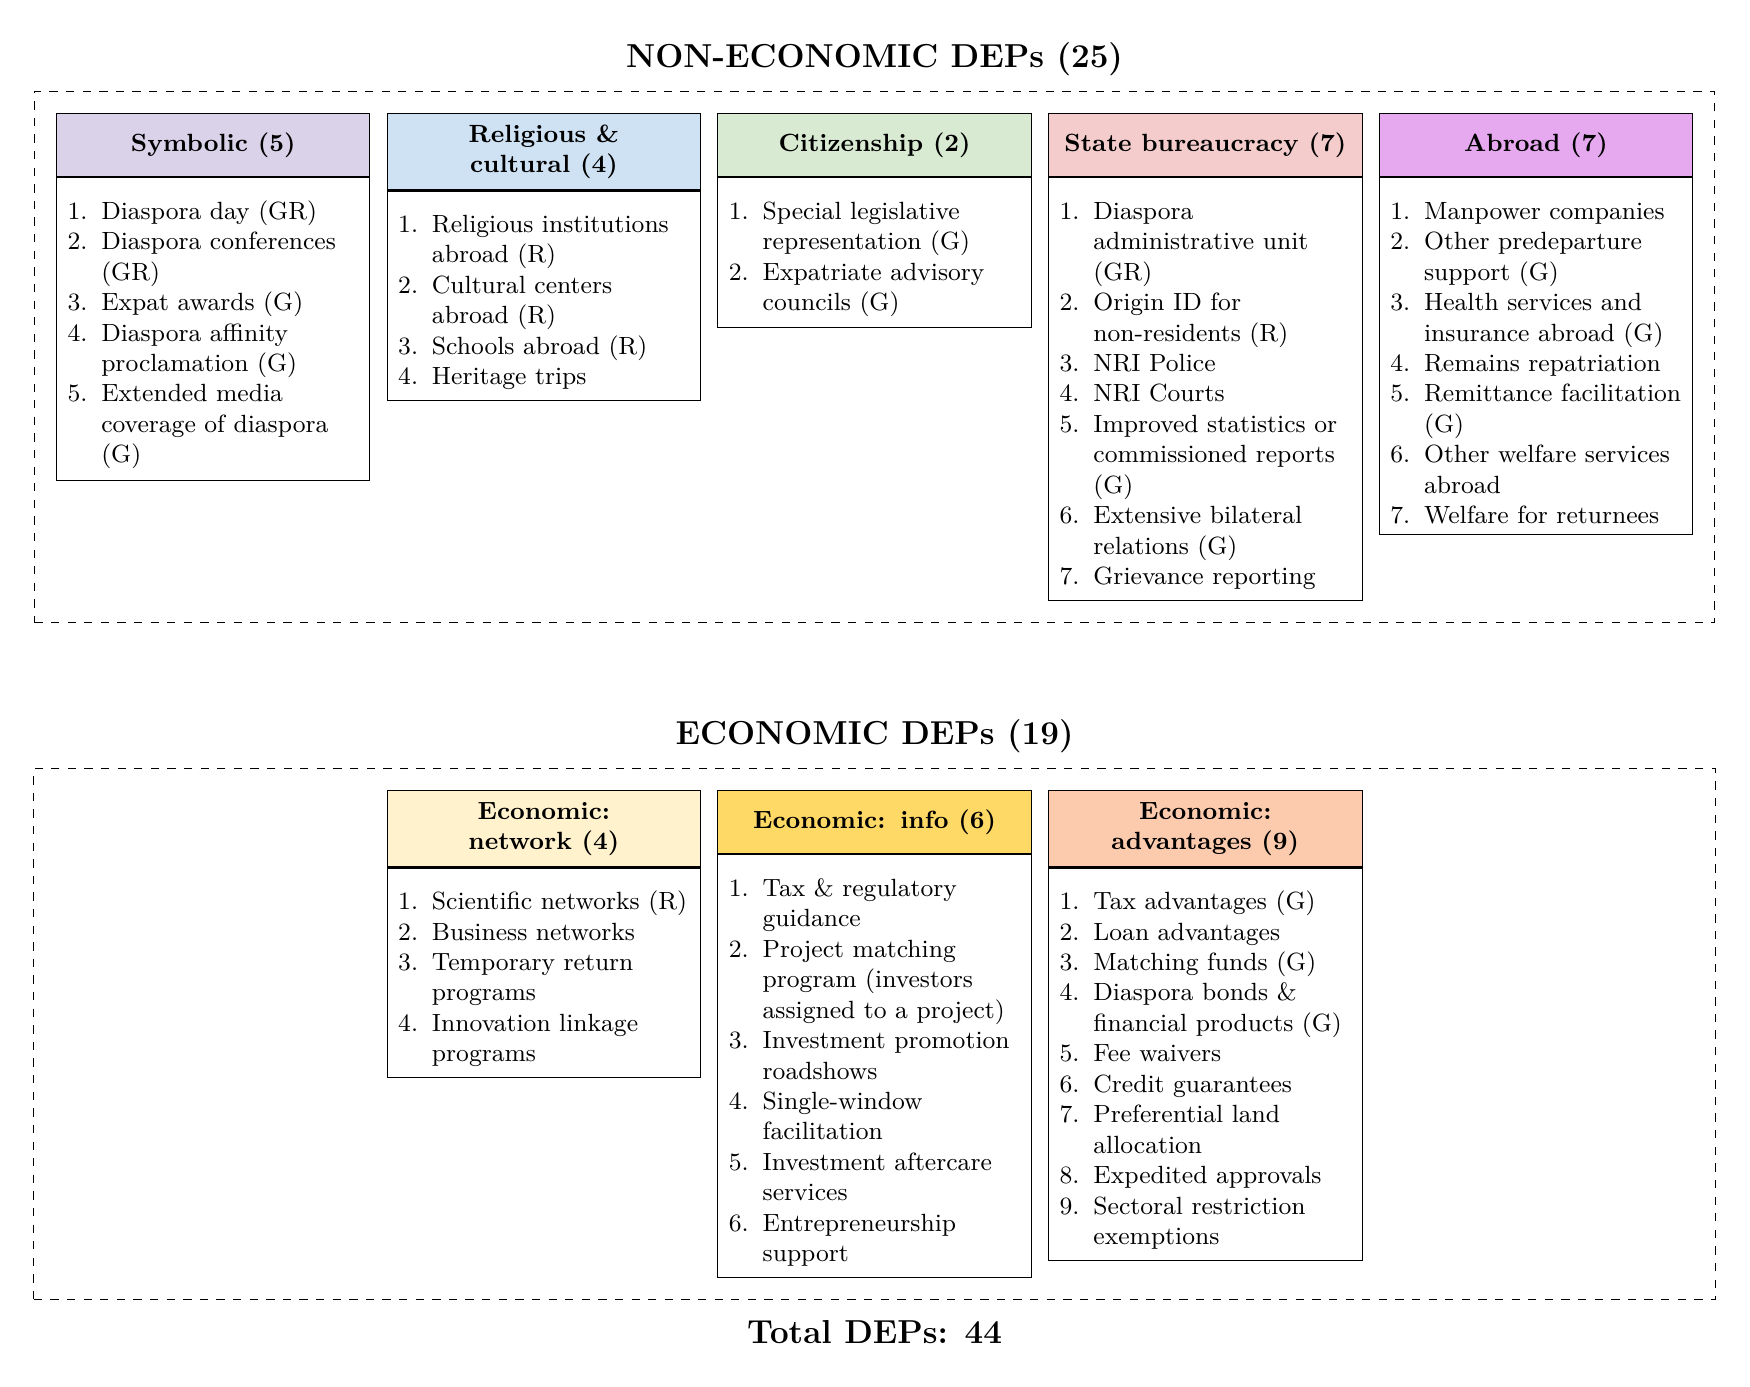
\includegraphics[width=\linewidth]{dep_sources.png}
    \caption{All 44 diaspora engagement policies, by category}
    \label{fig:deps_list}
    \begin{minipage}{\linewidth}\footnotesize \textit{Notes:} (G) indicates the DEP was used in \citet{gamlen_emigration_2008}, (R) indicates the DEP was used in \citet{ragazzi_comparative_2014}, two definitive works on DEP classification, and (GR) indicates the category was used in both. Unlabeled DEPs are the author's own classification. Some DEPs have been moved to different categories than in either work to best accommodate these 8 expanded categories.\end{minipage}
\end{figure}

\begin{figure}[htbp]
    \centering
    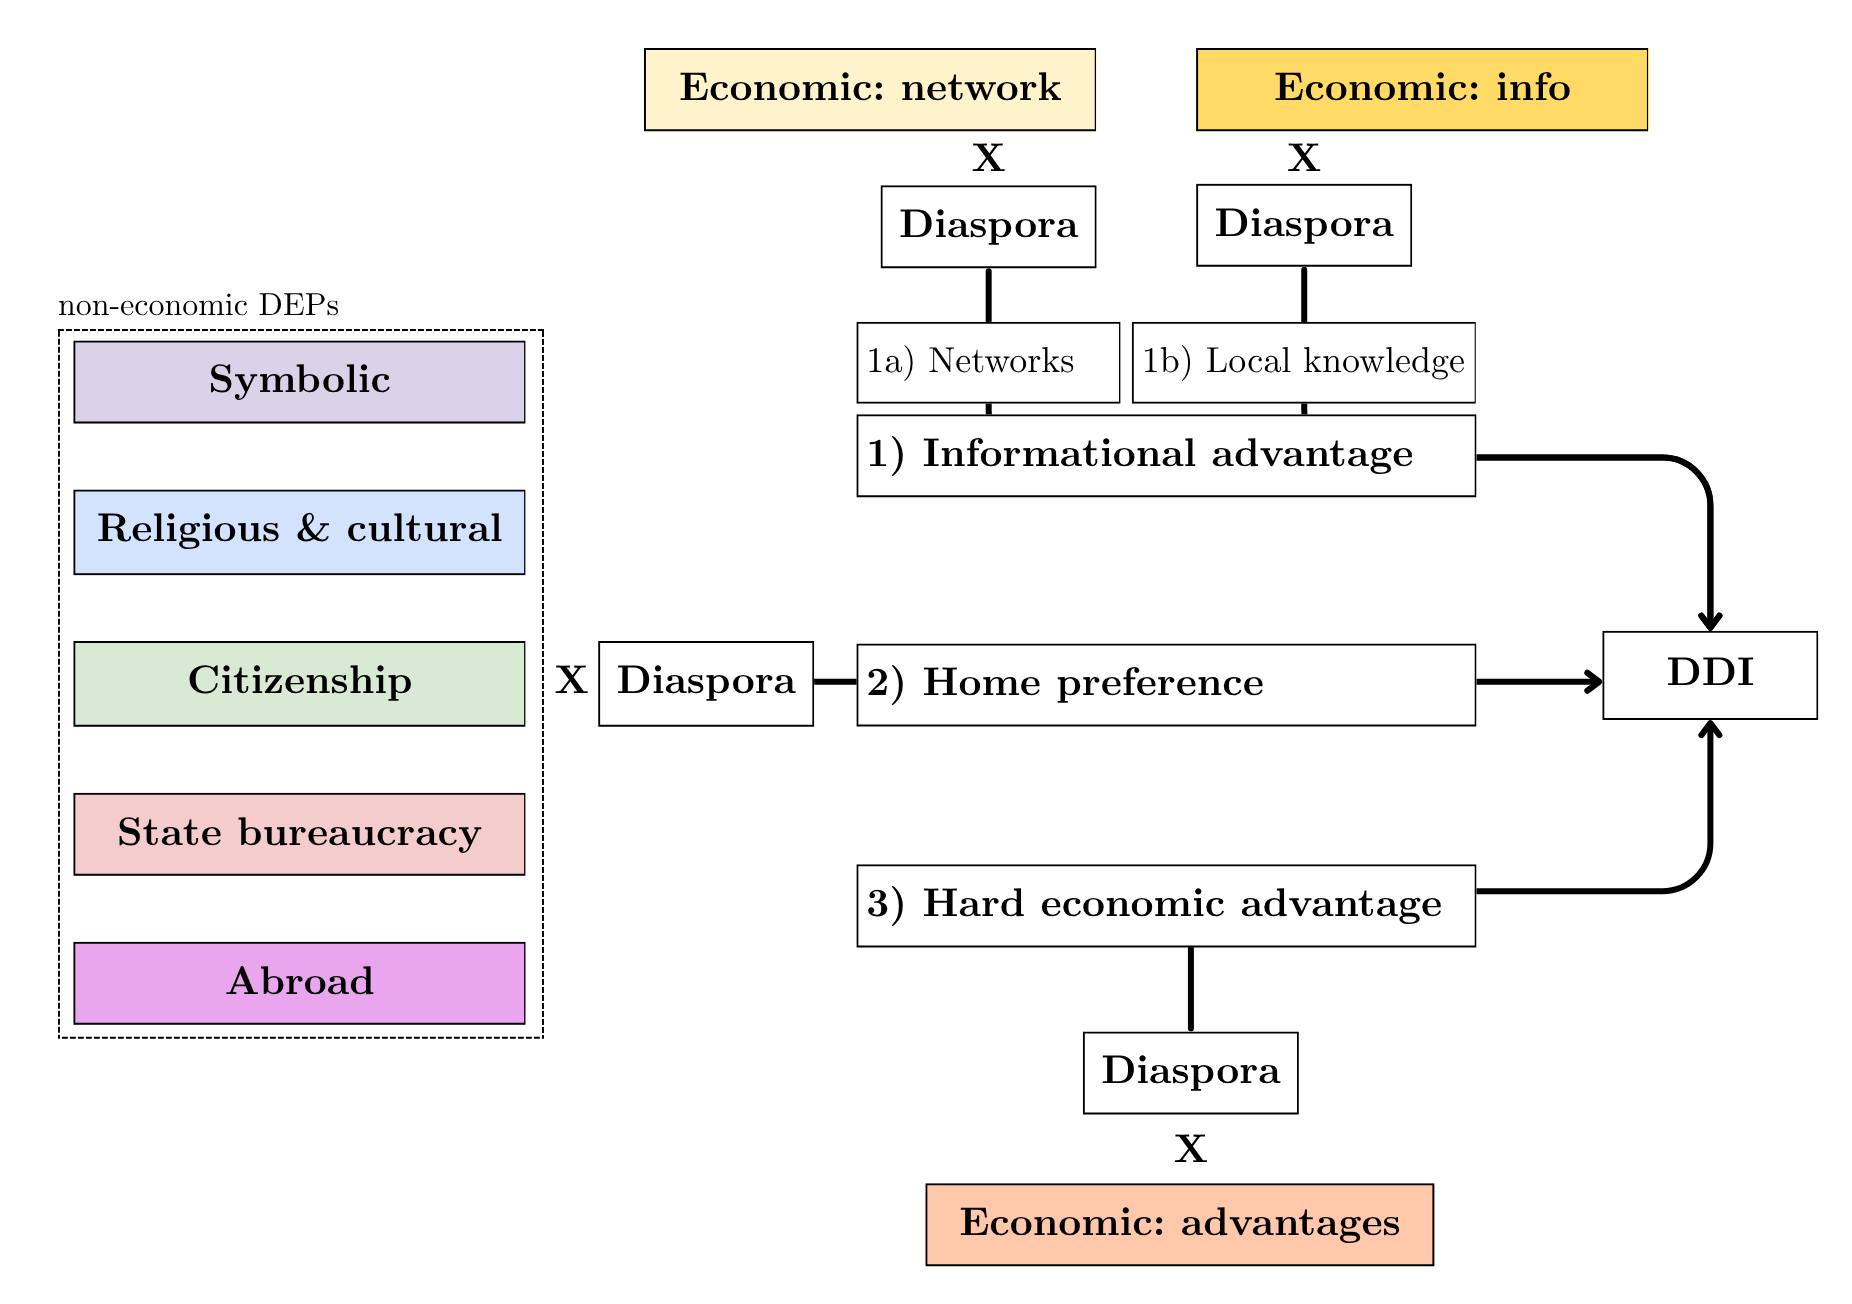
\includegraphics[width=\linewidth]{var_diagram.png}
    \caption{Mechanisms of diaspora direct investment and where DEPs fit in}
    \label{fig:variable diagram of pathways}
    \begin{minipage}{\linewidth}\footnotesize \textit{Notes:} DEPs interact with diasporas, meaning that they are only effective insofar as they attract any diaspora.\end{minipage}
\end{figure}


It is common practice in public sector economics to analyze policy at both the extensive margin (``does a state have a policy?'') and intensive margin (``how deeply implemented is the policy?''). Two hypotheses naturally result from this:

\begin{quote}
\textbf{$H_1$: As localities adopt any DEP, the positive effect diasporas have on FDI to that locality increases.}

\textbf{$H_2$: As localities' number of DEPs increases, the positive effect diasporas have on FDI to that locality increases.}
\end{quote}

The core of any FDI decision is, at the end of the day, how lucrative and feasible an opportunity is. As \citet{dunning_eclectic_2000} writes, firms invest where the combination of location advantages and internalization makes foreign production more valuable than the alternatives. Diaspora attachment can help bring a state into consideration, but an investor still must decide whether the project is profitable, legally possible, administratively feasible, and worth the risk. This implies that DEPs should be most effective when they reduce concrete transaction costs: information costs, such as not knowing which state incentives apply; bureaucratic costs, such as not knowing which official can resolve a problem; legal and regulatory costs, such as uncertainty about tax treatment or nonresident investor status; and trust costs, such as doubts about whether a local partner will follow through.

We can therefore rank DEPs in order of theoretical economic advantage. Non-economic DEPs should provide the least. Economic network DEPs, though useful at alerting investors to opportunities, are a more indirect way of providing informational advantage than soft facilitation DEPs. Both should provide less economic advantage than DEPs that lift regulatory barriers for diaspora members and fundamentally change their profit equation:
\[
\text{NonEconomic} < \text{Network} < \text{SoftFacilitation} < \text{HardAdvantage}
\]
This gives us our final hypothesis:

\begin{quote}
\textbf{$H_3$: As the economic advantage provided by a DEP increases, its impact on DDI becomes more positive.}
\end{quote}

Finally, the theory implies that DEP effects should vary by sector. If DEPs work by reducing information costs, trust costs, and bureaucratic uncertainty, then their effects should be strongest in sectors where those barriers matter most and where diaspora members have the most relevant knowledge. Knowledge-intensive sectors, especially ICT, are a natural place to expect stronger effects because they rely heavily on skilled labor, tacit information, professional networks, and confidence in local capabilities. In contrast, sectors driven primarily by natural resources, very large capital expenditure, or standardized production may depend less on diaspora-specific information. Therefore, while $H_1$--$H_3$ are stated generally, I expect the strongest results in ICT and other knowledge-intensive forms of FDI rather than in all FDI pooled together.

%==============================================================================
\section{Setting: Indian States and the US Diaspora} \label{sec:setting}
%==============================================================================

\subsection{Why India?}

It is incredibly difficult to do a multi-country study on subnational DEPs. Even with a host of fixed effects, any such study would require controlling for time-varying differences between countries that may affect both DEPs and DDI: adoption of other policies, spikes in corruption, or sectoral booms that disproportionately affect high-diaspora countries. Any empirical study must therefore begin with a single DDI source country and a single recipient country. In Online Appendix Section~\oaref{sec:oa_roadmap}, I lay out five filters a case must pass: the country must have subnational diasporas that see themselves as separate and that are measurable by language; its administrative units must map closely to those languages; some of those units must actually have DEPs; there must be no simultaneous nation-wide turn-on of those DEPs; and the units must receive enough FDI to make non-noisy inferences. Of the countries that pass, India and China provide the two most promising cases. This paper focuses on India for two reasons. First, there are more Indian subnational units that can be investigated: eight Indian states present real promise, while only two full Chinese provinces (Hunan and Jiangxi) stand up to confounding, and neither Xiang nor Gan are recorded in most FDI-sending-country census data. Second, India's policies largely evolved in contestation with the central Indian state \citep{sharma_partisan_2020}, and as such demonstrate more heterogeneity in policy design than China's, where Beijing supplied the framework for many provincial policies \citep{liu_chinas_2016}.

The United States is the natural FDI sending country. Over 2005--2017, the US sent 35\% of all inward FDI projects to India; the next largest was the UK, with 10\%. The US also has incredibly granular yearly data on languages through the American Community Survey (ACS), it has the largest combined population of non-citizen Persons of Indian Origin and Non-Resident Indians (5.4 million), and past studies have shown that US FDI abroad is positively correlated with the presence of migrants from the host country \citep{javorcik_migrant_2011}.

\subsection{Which states?}

India has many languages, with Indo-Aryan languages in the north and Dravidian languages in the south, and diaspora members tend to self-divide and identify along those linguistic lines \citep{sahoo_issues_2006, gautam_indian_2013}. Though some languages map to only one state, there are still many exceptions. I include a state only if it has one single dominant language, that language is not significantly spoken in any other Indian state or in another country, and the language is recorded in ACS data (Figure~\ref{fig:statesbylang}; Online Appendix Tables~\oaref{tab:language_fdi_sample}--\oaref{tab:language_fdi_a4} rate all 28 states and 8 union territories on each criterion).

One edge case was Andhra Pradesh. In 2014, the inland parts of Andhra were split to form Telangana. Both states are still Telugu-dominant, and diaspora from both states interact as one single community. As such, Andhra Pradesh is included in our sample up to the year 2013, and thereafter dropped. Four states had languages that cross national borders, and whether to include them depends on what share of their US diaspora comes from India. Indian Punjabis are routinely around 10 times more numerous in the US than Pakistani Punjabis, and Tamil speakers in the US are almost entirely India-born, so both stay in the sample. Bengalis of Indian origin are outnumbered roughly three to one in the US by Bengalis of Bangladeshi origin, so West Bengal is only included in samples of first-generation immigrants born in India. Almost no Nepali speakers in the US were born in India, so Sikkim is dropped. This leaves a sample of 8 states: Tamil Nadu, Kerala, Karnataka, Maharashtra, Andhra Pradesh (before 2014), Gujarat, Punjab, and West Bengal (first-generation samples only).

\begin{figure}[htbp]
    \centering
    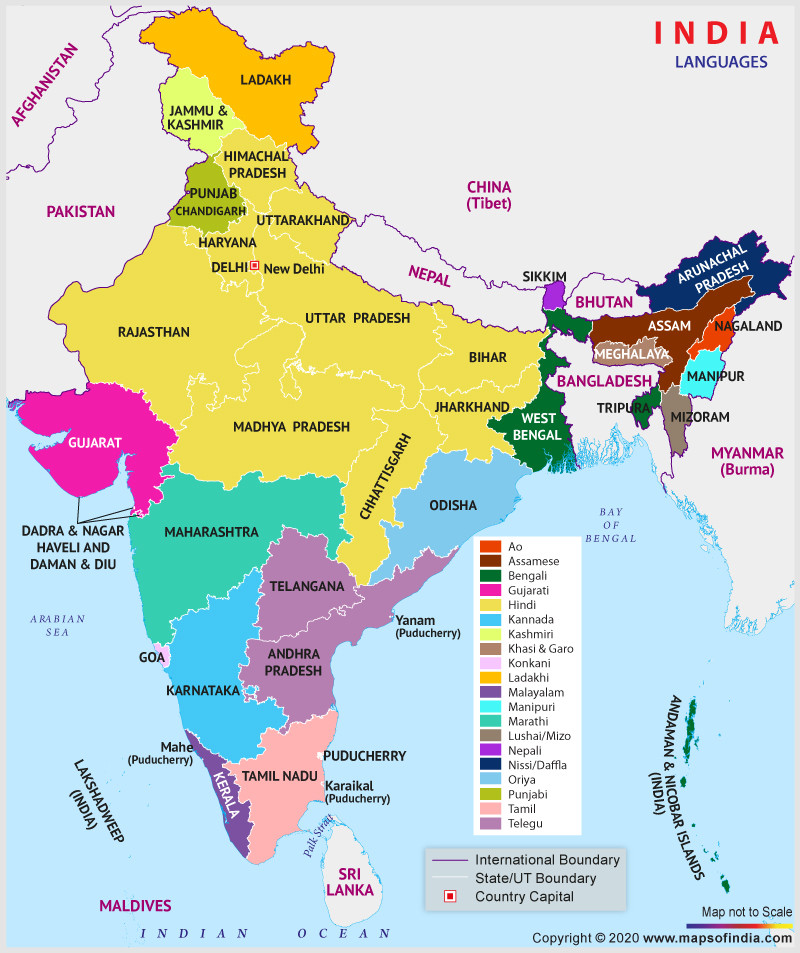
\includegraphics[width=0.85\linewidth]{states_by_language.png}
    \caption{States and union territories of India by dominant language}
    \label{fig:statesbylang}
    \begin{minipage}{0.85\linewidth}\footnotesize \textit{Notes:} States are colored by their most-spoken language, which does not reach a majority in some states. Source: \citet{noauthor_languages_nodate}.\end{minipage}
\end{figure}


\subsection{Do Indian states have real DEPs?}

Before spending a long time coding DEPs, it is wise to ask whether they are just names in newspaper announcements or whether they truly exist and do real work. DEPs have become essential in the minds of many state decision makers. In Kerala, NORKA has been a top-level department since 1996, and has been given its own section almost every year since 2001 in the Chief Minister's annual budget speech. In 2016, when Prime Minister Narendra Modi wanted to merge the national Ministry of Overseas Indian Affairs into the Ministry of External Affairs, Kerala Chief Minister Oommen Chandy publicly denounced the move as an ``insult to the whole NRI community'' \citep{ttn_team_kerala_2016}.

Policymakers also put their money where their mouths were (Figure~\ref{Budget}). From 2005 to 2017, Kerala multiplied its DEP budget more than 4 times, from 1,881 lakhs to 8,205 lakhs (2023 INR), equivalent to about \$10 million in 2026 USD. Punjab multiplied its budget 220 times, from 158 lakhs to 34,952 lakhs (\$41 million). From 2010, when it first created a DEP agency, to 2017, Tamil Nadu multiplied its DEP budget from 3,268 lakhs to 17,246 lakhs (\$20 million). The only state with budget data that did not see as large an increase was Andhra Pradesh, which went from 166 lakhs in 2008 to 253 lakhs in 2013 before its partition. Sources for each state's budget are in Online Appendix Section~\oaref{sec:oa_states}.

\begin{figure}[htbp]
    \centering
    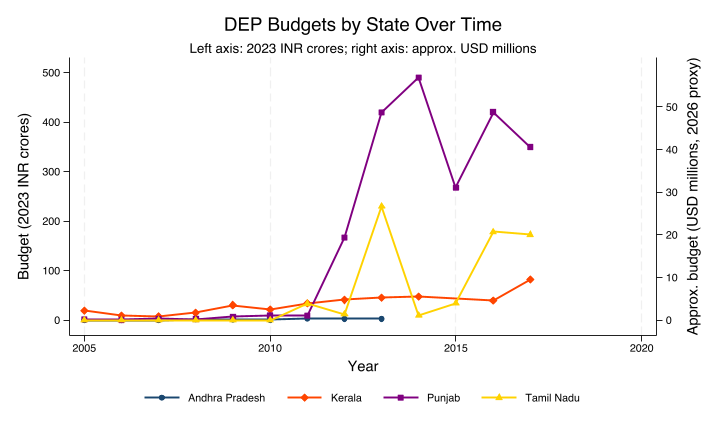
\includegraphics[width=0.85\linewidth]{4_3_fig4_dep_budgets_by_state.png}
    \caption{DEP budgets by state, 2005--2017}
    \label{Budget}
    \begin{minipage}{0.85\linewidth}\footnotesize \textit{Notes:} Created by author using official budgetary sources from Indian states. Some states with DEPs during this period are not shown (e.g. Gujarat) simply because their budgetary documents were not available, not because they did not have DEP line items.\end{minipage}
\end{figure}

These large investments have allowed DEPs to leave a genuine imprint in the migrant consciousness. A 2023 study conducted for NORKA, India's oldest state-level diaspora engagement agency, found that awareness of some NORKA programs is nearing 30\% of all emigrant households, with 29.7\% being aware of the Non-Resident Keralite ID Card and 26.3\% being aware of certificate attestation programs \citep{rajan_kerala_2023}. Evidence from Facebook also shows that DEPs have reached a large number of individuals: at the time of writing, NORKA Roots had 113 thousand followers and the Non-Resident Gujaratis' Foundation had 76 thousand, which rivals Indian national ministries like the Ministry of Law and Justice (19 thousand followers). This qualitative evidence that DEPs are prominent in the minds of lawmakers, receive real investment, and in turn are prominent in the minds of migrants means that DEPs are more than just ``paper programs.'' Budget speeches also show that policymakers across states share the primary goal of investment but differ in their secondary goals. In Kerala, budget sections on the diaspora are titled ``Welfare of Non-Resident Keralites'' \citep{isaac_government_2016}; in Punjab, DEP spending sits under ``Other Rural Development Programs'' \citep{finance_department_punjab_detailed_2013}. States whose DEPs align with the Kerala model of more welfare policies may have very different outcomes on FDI than those whose DEPs align with a more economic model.

%==============================================================================
\section{Data} \label{sec:data}
%==============================================================================

The unit of observation is a US metro area $m$, Indian state $s$, and year $t$, from 2005 to 2017. Each observation records the size of state $s$'s diaspora in metro $m$, the number of FDI projects from $m$ to $s$, and the DEPs state $s$ had in place. Online Appendix Section~\oaref{sec:oa_measurement} discusses each measure's validity and reliability in more detail.

\subsection{FDI}

FDI comes from all greenfield FDI projects to India in the fDiMarkets database, which records the date, source US city, destination Indian state, and sector of every project. I convert source cities into MET2013 metro areas through a spatial join. Following \citet{desbordes_effects_2017}, who note that FDI values mix together different kinds of transactions and miss real investment funded locally, I use project counts as the outcome. fDiMarkets also estimates capital investment and jobs, but both tend to spike with single large projects: Gujarat's 2015 spike is due to SunEdison's \$4 billion photovoltaic investment, 4 times larger than the next largest investment in the data \citep{inc_sunedison_nodate}.

It would be tempting to measure DDI directly by coding investors' names as Indian or not. Unfortunately, name data are blank for 34\% of projects, people with Indian names may not identify with the diaspora, the people named in announcements may not be the final decision makers, and even the best name-based algorithms identify an Indian state of origin with only around 80\% accuracy \citep{dhingra_instate_2023}. Most fundamentally, our theory is not about what percentage of DDI was by ``diaspora decision makers,'' but rather what the effect of the overall size of a diaspora on investment is by virtue of attributes that all scale with size: networks, knowledge of home region, home preference. I therefore draw from \citet{leblang_familiarity_2010}'s measure of DDI instead: I regress FDI on diaspora size and treat that relationship as DDI.

The name data can still give us directional answers about whether this construct of DDI is valid. The investors in the dataset had job titles largely recorded as President, C-suite, or heads of Indian divisions of companies, at both large multinationals and smaller firms, including startups led by diaspora entrepreneurs. Running their names through a model that predicts geographic origin from last names \citep{dhingra_instate_2023}, I find that around half of the FDI investors had Indian names and about a third of all projects were undertaken by them (Figure~\ref{fig:indian_names}). This is a robust finding for the idea that diaspora members in this dataset do influence investment decisions.

\begin{figure}[htbp]
    \centering
    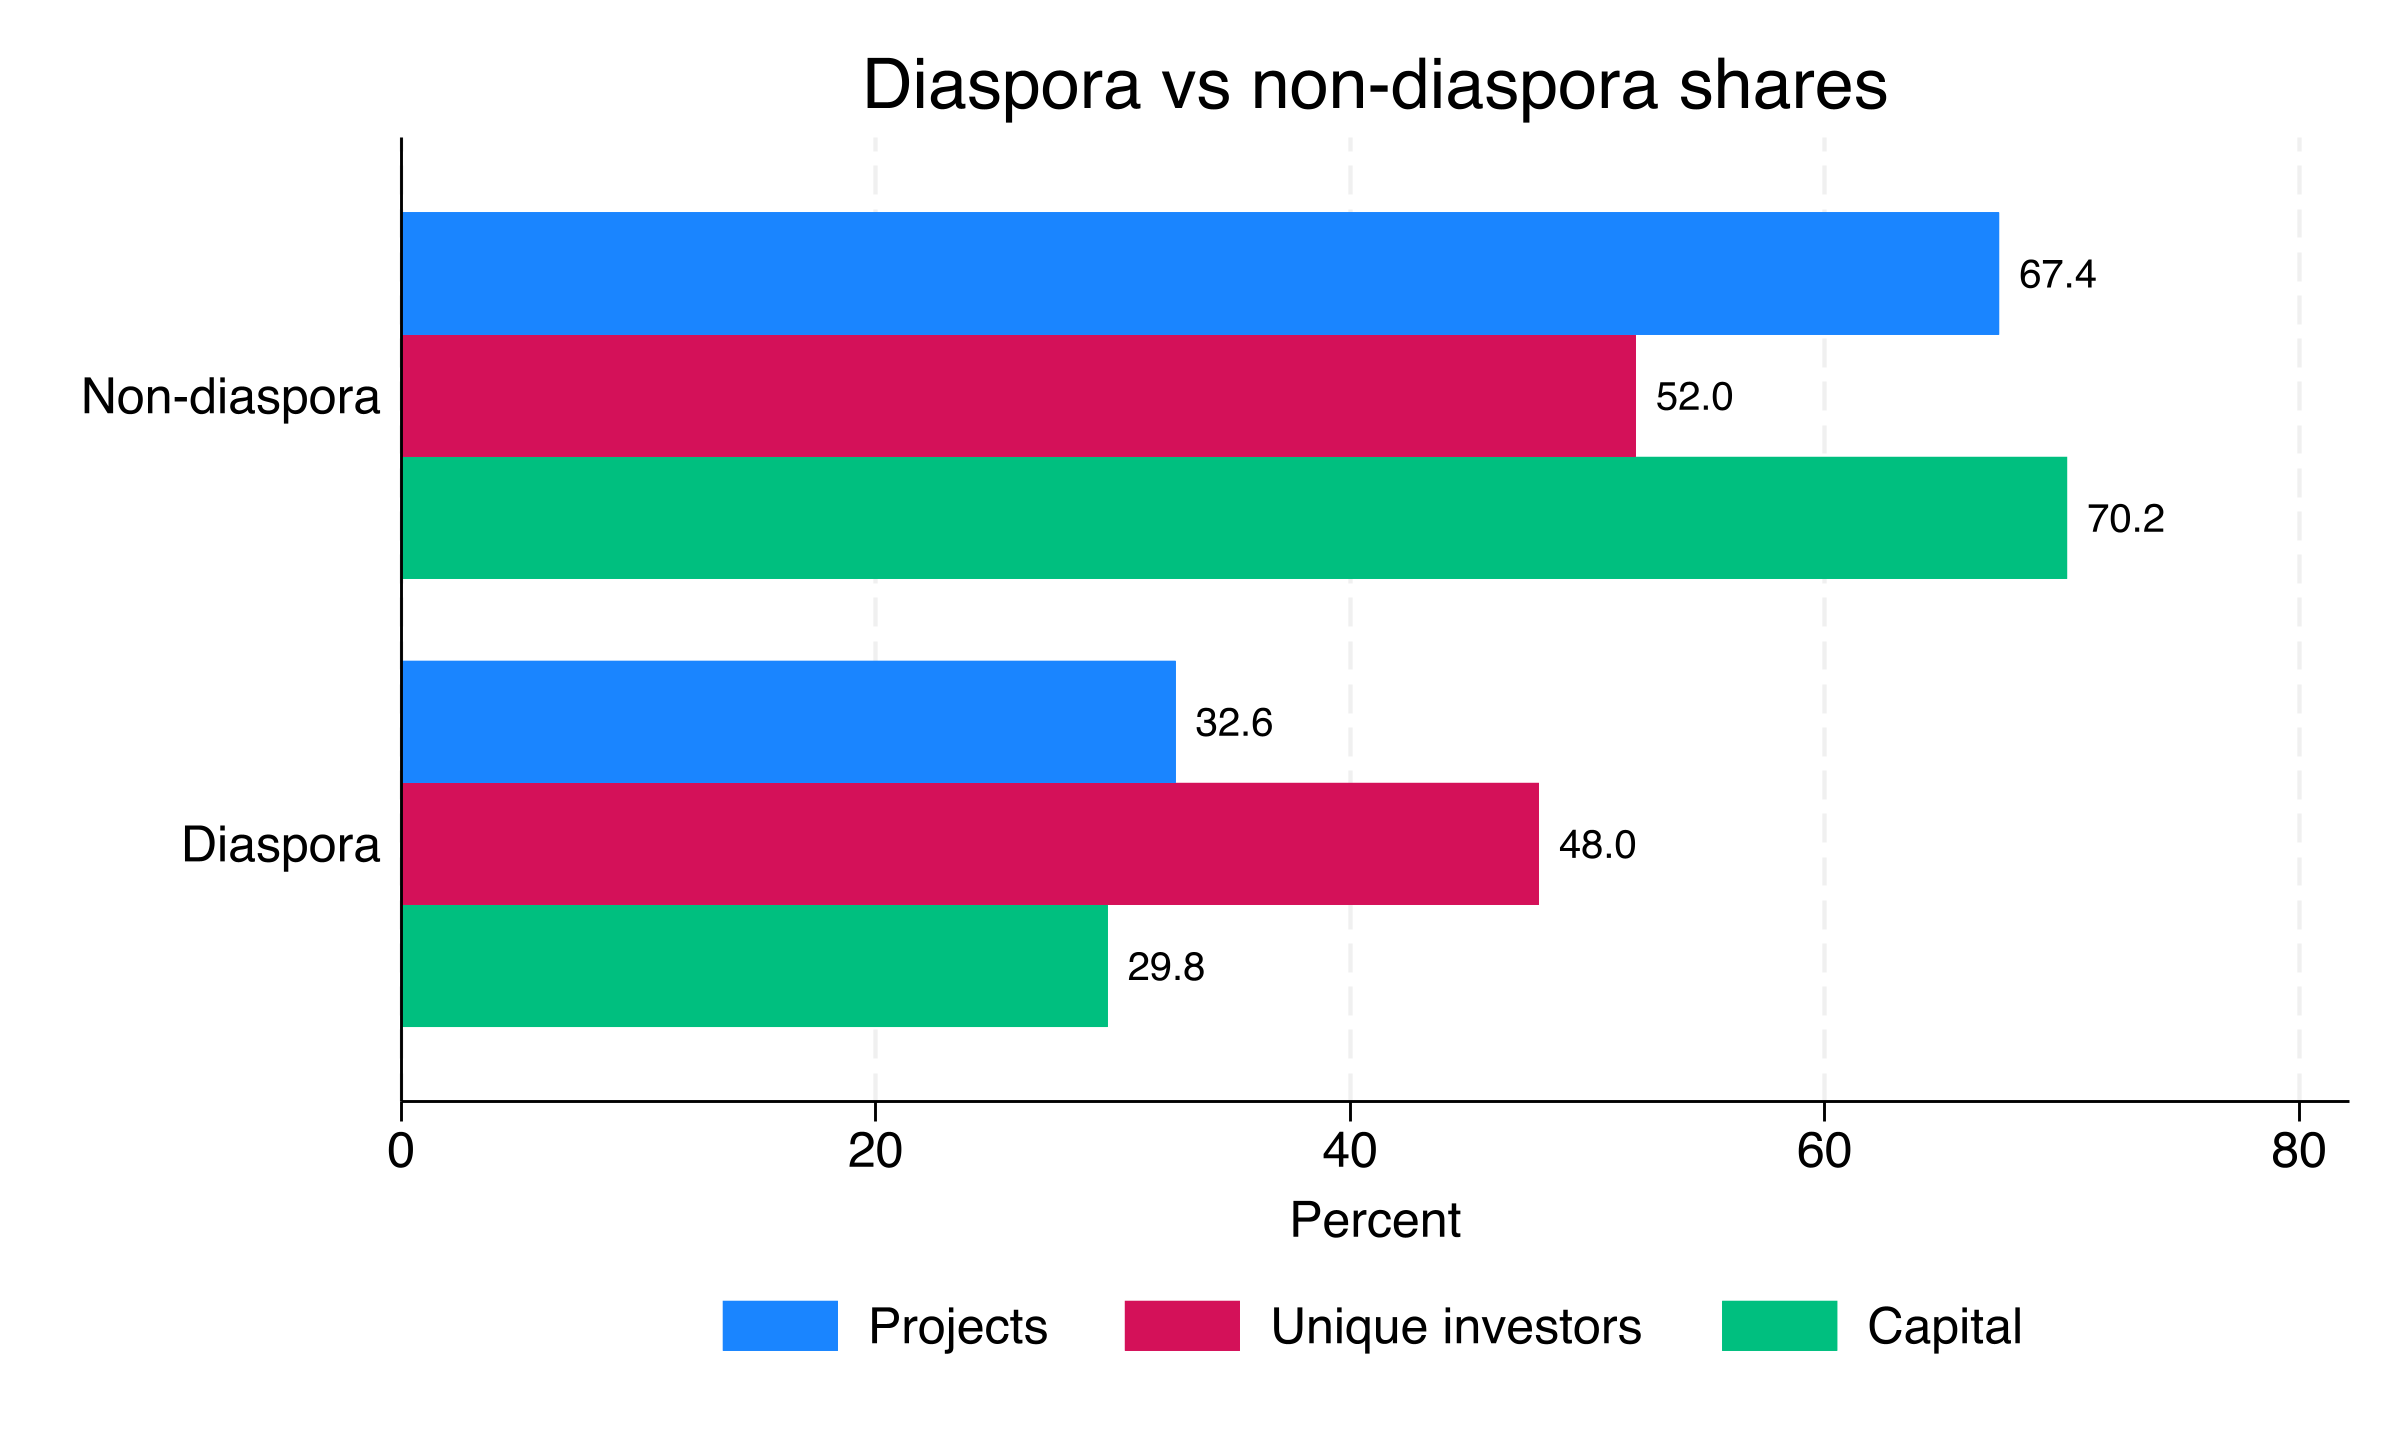
\includegraphics[width=0.7\linewidth]{4_6_fig5_indian_name_shares.png}
    \caption{Projects, investors, and capital from investors with possibly Indian names}
    \label{fig:indian_names}
    \begin{minipage}{0.7\linewidth}\footnotesize \textit{Notes:} Shares of all US-to-India projects, unique named investors, and capital investment, by whether the project's first listed contact has a possibly Indian name. Source: fDiMarkets.\end{minipage}
\end{figure}

Figure~\ref{fig:fdi_projects} shows project counts by state. In a confirmation of data fidelity, they clearly show the effect of India's 2005 FDI liberalization, with a large spike in 2006 that soon tapers off. Each state receives at least 5 projects a year and some receive 20--40, which is enough to make inferences. ICT is the largest sector by far, at 37.5\% of all projects, and roughly half of projects in earlier years.

\begin{figure}[htbp]
    \centering
    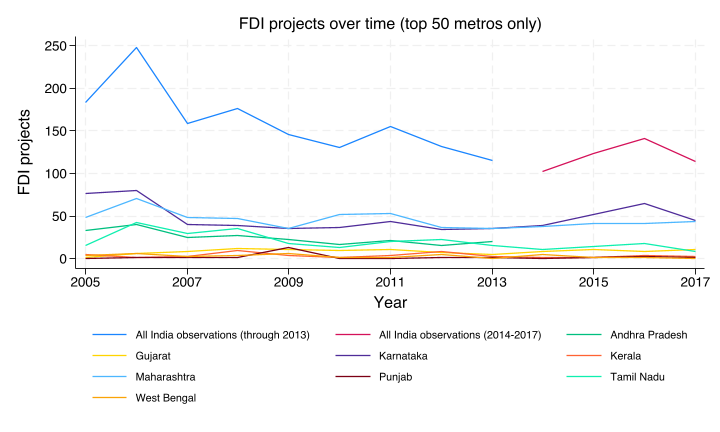
\includegraphics[width=0.85\linewidth]{4_1_fig6_fdi_projects_by_state.png}
    \caption{FDI projects from US metros by Indian state, 2005--2017}
    \label{fig:fdi_projects}
    \begin{minipage}{0.85\linewidth}\footnotesize \textit{Notes:} Projects from each diaspora's top 50 US source metros, with an all-India line split at Andhra Pradesh's 2014 bifurcation. Source: fDiMarkets.\end{minipage}
\end{figure}

\subsection{Diasporas}

Diasporas come from the US Census Bureau's 1\% samples, as processed by IPUMS. I use the LANGUAGE variable as a measure of subnational diaspora, with those that report speaking a certain language most at home being associated with a certain Indian state. LANGUAGE is only available yearly from 2005 onward, which is when our observation starts. There is a gap between this indicator and the construct of ``subnational diaspora'': Telugu diaspora members could be disproportionately likely to speak another language at home with their kids, or Tamil second-generation immigrants could be disproportionately likely to stop using Tamil and assimilate, and both language self-selection and intergenerational language loss are well documented \citep{escobar_indian_2022}. Still, LANGUAGE is our best and realistically only way of identifying subnational diasporas.

One way to mitigate this validity threat is, following the logic of \citet{mayda_refugees_2022}, to disaggregate the diaspora into metro areas. If we simply use the diaspora in the entire US, we would be comparing the effect of Gujarati non-resident IDs on Gujarati speakers across the entire US with the effect of Keralite non-resident IDs on Malayalam speakers across the entire US, which would likely be very biased by these language measurement issues. If we instead compare Gujarati speakers in Los Angeles with Gujarati speakers in New Jersey, a lot of those problems go away. Metro disaggregation also lets us apply metro-state pair fixed effects, removing all time-invariant differences in what kind of diaspora members live where: higher-educated Gujaratis may self-select into Silicon Valley, and a Gujarati who settles there is more likely to go into tech than her twin who settles in Charlottesville.

Metro area definition matters because undercounting or overcounting a metro area could skew those crucial fixed effects. Say for some reason we treated Cupertino as separate from the Bay Area. Then, because of all the Apple employees in Cupertino, we would underestimate the fixed effects for the Bay Area, and overestimate them for whatever metro we lump Cupertino with. IPUMS offers three metro measures; I use MET2013, which applies the 2013 Office of Management and Budget delineations across all years and does not identify any areas where the sum of omission and commission errors would be 15\% or more \citep{noauthor_ipums_nodate}. MET2013 is preferable to the newer MET2023 because our analysis stops in 2017, and to METAREA because METAREA changes its delineations with each decennial Census and leaves out many metro residents.

Because these are 1\% samples, small metro areas carry huge sampling variation in their yearly population estimates. I therefore restrict the analysis to each diaspora's top 50 US metros. Our results therefore apply to large metro areas, but this is a relatively minor concern because Indian subnational diaspora members tend to agglomerate: nearly 25\% of Gujaratis live in a single metro area (Edison, New Jersey). I build samples across several cleavages: generation (first-generation, i.e. born in India, versus all generations), education (college degree versus all), age (25 and over versus all adults), and occupation (ICT workers versus all). Table~\ref{tab:samples_by_n} shows the number of observations in the four main samples.

\begin{table}[htbp]
\centering
\caption{Samples by number of observations}
\label{tab:samples_by_n}
\begin{tabularx}{\textwidth}{@{}l Y r@{}}
\hline
Sample & Description & Distinct metro $\times$ state $\times$ year observations \\
\hline
Sample 1 & First-gen, high-edu, ICT FDI & 4919 \\
Sample 2 & First-gen, high-edu, all FDI & 4919 \\
Sample 3 & First-gen, all people, all FDI & 5058 \\
Sample 4 & All-gen, all people, all FDI & 4584*\\
\hline
\multicolumn{3}{@{}>{\RaggedRight\arraybackslash}p{\dimexpr\linewidth-2\tabcolsep\relax}@{}}{\footnotesize *Note: Sample 4 is smaller because it excludes West Bengal (we are unable to make reliable inferences about Bengali speakers without a birthplace of India, as most Bengali-Americans are born in Bangladesh).} \\
\end{tabularx}

\end{table}


\subsection{Diaspora engagement policies}

The DEP dataset is an original dataset of 104 state-year observations (8 states across 13 years), with 44 DEPs coded as dummies. I coded a DEP as 1 only if it met three conditions. First, the policy was implemented by the state government itself, which excludes NGOs, business councils, and cultural organizations even when they receive state funding. Second, the policy was exclusively targeted towards the subnational diaspora. Many state investor-promotion policies, like single-window facilitation portals, were undoubtedly used by the diaspora, but were not designed to give them any special advantage. Third, the DEP did not just exist on paper, but was actually carried out. Karnataka is the clearest example of why this matters: though it has a DEP website full of promises made in 2016, not a single one was ever carried out. I looked through news announcements, budget speeches, and NRI agency websites for announcements of new policies, then looked for confirmatory evidence from government budgets, official paper trails, the Internet Archive, or national government documents, and built state-year audit tables listing the first year each policy turned on and the evidence for it. Secondhand accounts via news articles and social media were helpful, but I would not code a policy as 1 using those accounts alone unless I found two or more corroborating accounts of the same policy. The full codebook and process are in Online Appendix Section~\oaref{sec:oa_deps}.

Despite this process, there are still remaining threats to validity and reliability. First, by coding only policies that were implemented by state governments themselves, I gained conceptual clarity, but I may also exclude policies that meaningfully shaped diaspora investment, like a state-backed business council or public-private investment forum. This is a conservative tradeoff: I prefer to measure a narrower construct clearly rather than include ambiguous quasi-governmental activities that blur the line between state policy and civil society. Second, dummy coding may flatten meaningful differences in policy intensity. Two states may both have diaspora investment facilitation programs, but one may have a staffed agency, clear application procedures, and regular outreach, while the other has only a lightly maintained webpage. The measure therefore captures the extensive margin of policy adoption more cleanly than the intensive margin of policy strength. Third, historical documentation is uneven across states and years, which creates a risk that observed differences in DEPs partly reflect differences in surviving records. Fourth, some policies sit near the boundary between categories: an investment roadshow may also involve business networking, and a diaspora conference may include grievance redressal. I coded policies by their clearest implemented function, but because I am the sole coder, some judgment-based inconsistencies may remain.

Figure~\ref{fig:total_deps} shows that the total number of DEPs per state increases quite substantially over 2005--2017, but unevenly: Kerala and Punjab accumulate the most, while Maharashtra and West Bengal adopt none in this period. Adoption is staggered rather than tied to any single national date. I also structured the policy buckets to be as mutually exclusive and collectively exhaustive as possible, because policies that are essentially the same thing would always turn on together and make inferences unstable. Co-adoption is rare: very few policy pairs have a Jaccard similarity above 0.1, and the largest same-year package contains three DEPs (Online Appendix Section~\oaref{sec:oa_deps}).

\begin{figure}[htbp]
    \centering
    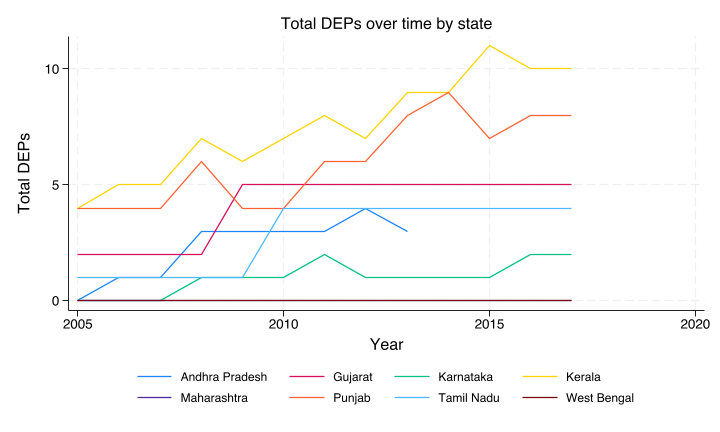
\includegraphics[width=0.85\linewidth]{4_1_fig7_total_deps_by_state.png}
    \caption{Total active DEPs by Indian state, 2005--2017}
    \label{fig:total_deps}
    \begin{minipage}{0.85\linewidth}\footnotesize \textit{Notes:} Number of the 44 coded DEPs active in each state-year. Andhra Pradesh stops in 2013 because of the state's bifurcation. Source: author's DEP dataset.\end{minipage}
\end{figure}

%==============================================================================
\section{Empirical Strategy} \label{sec:strategy}
%==============================================================================

\subsection{Estimation}

Following the extant literature on FDI, I estimate every model with Poisson pseudo-maximum likelihood (PPML). This is because the outcome is a count, this is a gravity setting, and the data have many zeros. A gravity model explains flows between two places as a function of connection and barriers: just like in physics, flows rise when two places are larger or more connected, and fall when barriers between them are higher. Here, the flow is the number of FDI projects from US metro $m$ to Indian state $s$ in year $t$, the connection is partly captured by the size of the relevant subnational diaspora in metro $m$, and the barriers are the informational, bureaucratic, legal, and familiarity costs of investing in a particular Indian state.

PPML's exponential mean means each covariate shifts the expected flow in percentage-like terms rather than adding a fixed number of projects, which fits FDI: a larger diaspora probably does not add the same number of projects to every metro-state pair, but changes the expected rate of investment proportionally. PPML also handles zeros, which are meaningful here. If Punjabi-heavy Los Angeles sends zero FDI projects to Punjab in 2009, that is substantively meaningful, and dropping it with a logged outcome would throw away exactly the information we need. Finally, PPML only needs the conditional mean to be correctly specified, not the full distribution, so it remains consistent with lumpy, overdispersed, heteroskedastic project counts \citep{santos_silva_log_2006}. I estimate all models with \citet{correia_fast_2020}'s ppmlhdfe.

For $H_0$, I estimate
\begin{equation}
E[Y_{mst} \mid X_{mst}] = \exp \bigl( \beta_1 \ln(1+Diaspora_{mst}) + \alpha_{m} + \delta_{st} \bigr),
\label{eq:h0}
\end{equation}
where $Y_{mst}$ is the count of FDI projects from US metro $m$ to Indian state $s$ in year $t$, $Diaspora_{mst}$ is the relevant diaspora population, $\alpha_m$ are metro fixed effects, and $\delta_{st}$ are state-year fixed effects. I run this on both the subnational diaspora and the broader Indian diaspora in each metro, then compare $\beta_1$ across the two. State-year fixed effects absorb all factors common to an Indian state in a given year. We cannot use metro-year fixed effects here because total Indian diaspora size only varies at the metro-year level and would be perfectly collinear with them, so for the sake of comparison both rows exclude them. Standard errors are clustered by metro-state pair. The $H_0$ results should therefore be read as descriptive rather than causal.

For $H_1$--$H_3$, I estimate
\begin{equation}
\begin{aligned}
E[Y_{mst} \mid X_{mst}] = \exp \Bigl( &\beta_1 \ln(1+Diaspora_{mst}) + \beta_2 DEP_{st} \\
&+ \beta_3 \left[\ln(1+Diaspora_{mst}) \times DEP_{st}\right] + \alpha_{ms} + \gamma_{mt} + \delta_{st} \Bigr),
\end{aligned}
\label{eq:h1}
\end{equation}
where $DEP_{st}$ is an indicator for any active DEP ($H_1$), a count of active DEPs ($H_2$), or a count of active DEPs in one category ($H_3$). Metro-state dyad fixed effects $\alpha_{ms}$ net out time-invariant bilateral factors like persistent metro-state affinity and historical business ties. Metro-year fixed effects $\gamma_{mt}$ capture metro-year shocks, like a tech boom in San Francisco. Because $DEP_{st}$ varies only at the state-year level, $\beta_2$ is absorbed by $\delta_{st}$; the theoretically relevant quantity is $\beta_3$, which tells us whether DEPs change how strongly diaspora size translates into FDI. Because DEPs are assigned at the state level, standard errors are clustered by Indian state. This leaves only 8 clusters, so inferences are fragile, and I emphasize effect direction, magnitude, and consistency rather than just significance.

To interpret $\beta_3$, note that a coefficient of $\beta_3$ means that when the DEP is on, doubling the diaspora is associated with approximately $2^{\beta_3}$ times as much FDI as the same doubling without the DEP (the approximation is close for all but very small diasporas, since the regressor is $\ln(1+Diaspora_{mst})$). A $\beta_3$ of 0.5, for example, implies $2^{0.5} = 1.41$, or 41\% more FDI from a diaspora doubling under the policy than without it.

The $H_1$--$H_3$ estimates are single-policy estimates: each model swaps one DEP measure into the DEP term. This is appropriate when the goal is a clean reduced-form estimate for one treatment at a time rather than a decomposition across overlapping treatments \citep{goldsmith-pinkham_estimating_2021}; with more than 40 policies, a model with all of them at once could not estimate individual effects well. Two features of the DEP data need care. Rare policies, adopted by fewer than 2 states or for fewer than 10 state-years, are much more like case-study contrasts than panel estimates, so I exclude them from the $H_2$ count and the $H_3$ categories. Bundling, where a state adopts several DEPs in one reform package, means that individual-policy and category coefficients should be read as reduced-form associations with policy types rather than fully separable effects of each instrument; this matters less for $H_1$ and $H_2$, where a bundled package is part of the treatment itself. Finally, ppmlhdfe drops singletons and separated observations, so every table reports the number of observations before and after those drops.

\subsection{Identification}

The identifying assumption is that after conditioning on dyad, metro-year, and state-year fixed effects, there are no omitted shocks correlated with the regressor of interest. I discuss three threats here and the rest in Online Appendix Section~\oaref{sec:oa_identification}.

The first is reverse causation: if states adopt DEPs in response to rising FDI, our estimates would reflect states with higher untreated paths, not the effect of DEPs. Three pieces of evidence make this unlikely. First, the states that adopt DEPs mostly do so 3--4 years after the 2005 FDI liberalization spike, and qualitative records show that only Gujarat framed its policies in terms of investment at all. In Andhra Pradesh, the contemporaneous architecture was centered on migrant welfare and protection; in Punjab, the 2008 NRI push was framed around solving NRIs' concrete problems with the state, pairing NRI police stations and fast-track courts with promises to support village schools and hospitals \citep{society_andhra_nodate, noauthor_nri_nodate}. Second, the states with the most extensive DEPs are those without much FDI (Kerala, Punjab, Gujarat), while those with a lot of FDI (Andhra Pradesh, Maharashtra, Tamil Nadu, Karnataka) adopt fewer DEPs. Third, several low-FDI states created diaspora administrative units in the 1990s and early 2000s, long before any FDI spike. Administrative units are logically the most intentionally created of any DEP, likely implemented only after intensive deliberation by high-level decision makers, so their timing is especially informative. Gujarat is the least clean case, since its 2009 initiatives were openly pro-business, but even there the official rationale was broad developmental mobilization of the diaspora rather than a response to rising FDI flows: the Non-Resident Gujaratis' Foundation's stated objectives stressed communication with overseas Gujaratis, addressing their social and cultural issues, and channeling their resources into Gujarat's general development effort \citep{noauthor_home_nodate}. Finally, many states' DEP administrations sit under migrant welfare (Andhra Pradesh, Tamil Nadu, Kerala) and rural development (Punjab) rather than investment. Any reverse causation issues are likely to be minimal.

The second is spillovers: one state's DEP might pull an investor away from another state, or a roadshow might raise awareness of India in general. This threat is limited because all DEPs in this dataset are subnationally targeted. A diaspora member is unlikely to attend an NRI Punjab Sammelan, use a Telugu grievance cell, or seek Kerala returnee assistance simply to learn about India in general. The safest interpretation is that the estimates capture whether DEPs help states attract more FDI from their own larger-diaspora dyads relative to smaller-diaspora dyads, not whether DEPs increase aggregate FDI to India.

The third is diaspora-skewed shocks that the fixed effects do not absorb. If Karnataka has a tech boom in 2011, San Francisco, with many Kannada speakers, might increase its FDI by a larger proportion per diaspora member than Cambridge, Massachusetts, even if both are tech hubs. The same is true of general growth shocks and non-diaspora investment policies whose effects scale with diaspora size. Natural controls such as state GDP, investment budgets, or non-DEP policy counts are bad controls here: they are plausibly mediators, post-treatment confounders, colliders, or close proxies for the outcome itself. Instead, Table~\ref{tab:ovb_signing_fe} signs the bias from each plausible omitted variable.

\begin{table}[htbp]
\centering
\caption{Most plausible remaining omitted-variable biases after metro-year, state-year, and dyadic fixed effects}
\label{tab:ovb_signing_fe}
\small
\begin{tabularx}{\textwidth}{@{}Y Z Z Z Y Y@{}}
\hline
Omitted variable $Z$ & Corr$(Z,D)$ & Corr$(Z,Y)$ & Sign & Biases estimate by & Magnitude \\
\hline
Diaspora-skewed state growth shock & Likely $+$ & Likely $+$ & $+$ & Overstates DEP effect & Moderate \\
Diaspora-skewed investment budget & Likely $+$ & Likely $+$ & $+$ & Overstates DEP effect & Large \\
Diaspora-skewed non-DEP policy package & Likely $+$ & Likely $+$ & $+$ & Overstates DEP effect & Large \\
Weakening diaspora responsiveness in treated pairs & Likely $+$ & Likely $-$ & $-$ & Understates DEP effect & Moderate \\
Strong substitute investment channels & Likely $-$ & Likely $+$ & $-$ & Understates DEP effect & Moderate \\
\hline
\end{tabularx}
\begin{minipage}{\linewidth}\footnotesize \textit{Notes:} $D$ is the regressor of interest, $\ln(1+Diaspora_{mst}) \times DEP_{st}$, net of the metro-state, metro-year, and state-year fixed effects. $Y$ is the FDI project count.\end{minipage}
\end{table}

On net, the results likely somewhat overstate the true influence of DEPs on diaspora FDI. This, combined with the small number of clusters, means we should be cautious about borderline-significant results in $H_1$--$H_3$. The estimates are best read as strong reduced-form, quasi-causal estimates: if positive, they tell us that after DEP adoption, FDI rises more in larger-diaspora dyads than in smaller-diaspora dyads.

The baseline samples give a cross-section of the cleavages above: first-generation diaspora with ICT FDI as the outcome, first-generation high-education 25+ with all FDI, first-generation 25+ with all FDI, all-generation 25+ with all FDI, and all-generation with all FDI. I break out ICT FDI because it is the largest sector by far, spanning 37.5\% of all projects.

%==============================================================================
\section{Results} \label{sec:results}
%==============================================================================

\subsection{Location-specific diasporas and FDI}

Table~\ref{tab:final_baseline_h0} tests $H_0$. Across all samples, the subnational diaspora is positively associated with FDI, with coefficients from 0.069 to 0.102. $\beta_1$ is largest for the first-generation ICT sample, but more precisely estimated in the all-FDI samples, which have more projects. Meanwhile, the national Indian diaspora is not significantly associated with FDI in any sample. $H_0$ is thus supported: in the Indian context from 2005--2017, subnational diasporas have a much stronger association with FDI than the national diaspora. The Gujarati population in Edison, the Telugu population in Dallas, or the Tamil population in the Bay Area carries location-specific information and attachment that a generic Indian diaspora measure does not capture, consistent with work showing that diaspora effects operate through familiarity, local knowledge, and transaction-cost reduction \citep{leblang_familiarity_2010, kugler_migration_2018, useche_highly_2020}. Although this result is descriptive, it is a useful validation: if national diaspora size had predicted state-level FDI just as well, the case for studying subnational DEPs would be weaker.

\begin{table}[!htbp]
\centering
\footnotesize
\setlength{\tabcolsep}{3pt}
\renewcommand{\arraystretch}{1.08}
\caption{H0: location-specific diaspora versus national Indian diaspora stock: baseline samples}
\label{tab:final_baseline_h0}
\begin{tabularx}{\textwidth}{@{}>{\RaggedRight\arraybackslash}X *{5}{>{\Centering\arraybackslash}X}@{}}
\hline
Specification & First-gen all diaspora, ICT FDI & First-gen 25+ high-ed, all FDI & First-gen 25+ all diaspora, all FDI & All-gen 25+ all diaspora, all FDI & All-gen all diaspora, all FDI \\
\hline
Subnational diaspora: exporter FE + importer-year FE & 0.102* & 0.069** & 0.084** & 0.072** & 0.076** \\
 & (0.055) & (0.033) & (0.035) & (0.037) & (0.037) \\
National Indian diaspora: exporter FE + importer-year FE & -0.123 & -0.184 & -0.212 & -0.028 & 0.120 \\
 & (0.344) & (0.204) & (0.210) & (0.206) & (0.206) \\
\hline
Raw sample N & 5058 & 4897 & 5025 & 4546 & 4584 \\
Projects, 2005--2017 & 790 & 2130 & 2125 & 2101 & 2109 \\
Total diaspora pop., 2005--2017 & 10968732 & 7021199 & 9867596 & 10785954 & 13763848 \\
e(N\_full) & 5058 & 4897 & 5025 & 4546 & 4584 \\
e(N) & 2529 & 3575 & 3669 & 3333 & 3350 \\
Dropped singletons & 2529 & 1322 & 1356 & 1213 & 1234 \\
Dropped separated obs & 0 & 0 & 0 & 0 & 0 \\
\hline
\fulltablenote{6}{Cells are coefficients on ln\_dias (or the national Indian diaspora), with SEs clustered by metro-state pair directly underneath. Fixed effects as listed in each row.}
\fulltablenote{6}{* p<0.10, ** p<0.05, *** p<0.01.}
\end{tabularx}
\end{table}


\subsection{DEP adoption}

Table~\ref{tab:final_baseline_table2_h1} tests $H_1$, and it is where the story becomes sharply sector-specific. The extensive-margin DEP result is concentrated in ICT FDI. The first column's coefficient on any DEP adoption is 0.196 and significant at the 1\% level. This implies that, after a state adopts any DEP, a doubling of the relevant diaspora is associated with about 15\% more ICT FDI than the same diaspora doubling would be associated with absent that DEP. That is a meaningful moderation effect: DEPs do not simply raise a state's FDI level mechanically, they make diaspora concentration more predictive of where ICT projects locate. By contrast, the all-FDI columns are all close to zero and insignificant. DEPs do not appear to make diasporas generally better at attracting every kind of FDI; they appear to make diasporas better at attracting ICT FDI. There is enough evidence to confirm $H_1$ for ICT FDI, while there is little evidence for non-ICT FDI.

\begin{table}[!htbp]
\centering
\footnotesize
\setlength{\tabcolsep}{3pt}
\renewcommand{\arraystretch}{1.08}
\caption{Any DEP adoption x diaspora: baseline samples}
\label{tab:final_baseline_table2_h1}
\begin{tabularx}{\textwidth}{@{}>{\RaggedRight\arraybackslash}X *{5}{>{\Centering\arraybackslash}X}@{}}
\hline
Specification & First-gen all diaspora, ICT FDI & First-gen 25+ high-ed, all FDI & First-gen 25+ all diaspora, all FDI & All-gen 25+ all diaspora, all FDI & All-gen all diaspora, all FDI \\
\hline
Any DEP adoption & 0.196*** & -0.020 & 0.003 & 0.008 & 0.001 \\
 & (0.059) & (0.034) & (0.029) & (0.026) & (0.027) \\
\hline
Raw sample N & 5058 & 4897 & 5025 & 4546 & 4584 \\
Projects, 2005--2017 & 790 & 2130 & 2125 & 2101 & 2109 \\
Total diaspora pop., 2005--2017 & 10968732 & 7021199 & 9867596 & 10785954 & 13763848 \\
e(N\_full) & 5058 & 4897 & 5025 & 4546 & 4584 \\
e(N) & 916 & 1937 & 1945 & 1773 & 1781 \\
Dropped singletons & 4142 & 2960 & 3080 & 2766 & 2797 \\
Dropped separated obs & 0 & 0 & 0 & 7 & 6 \\
\hline
\fulltablenote{6}{Cells are coefficients on ln\_dias x policy, with SEs clustered by Indian state directly underneath. All models include metro-state, metro-year, and state-year fixed effects. --- marks an interaction ppmlhdfe omits because it is not identified once singletons and separated observations are dropped.}
\fulltablenote{6}{* p<0.10, ** p<0.05, *** p<0.01.}
\end{tabularx}
\end{table}


\subsection{DEP intensity}

At the intensive margin (Table~\ref{tab:final_baseline_table3_h2}), the result becomes weaker but does not disappear. The ICT column again has the only positive and marginally significant coefficient. A coefficient of 0.084 means each additional support-screened DEP is associated with roughly 6\% more ICT FDI for a doubling of the relevant diaspora. Substantively, this suggests that the first policy, or the existence of a state diaspora apparatus at all, may matter more than the simple count of policies a state has. That is intuitive: one meaningful investment-facing doorway may matter more than a long policy list, especially if some policies are symbolic or welfare-oriented. DEP count is also a crude measure of intensity, treating a lightly maintained website and a well-funded facilitation program as equivalent. There is suggestive evidence for $H_2$ for ICT FDI, and again little evidence for non-ICT FDI.

\begin{table}[!htbp]
\centering
\footnotesize
\setlength{\tabcolsep}{3pt}
\renewcommand{\arraystretch}{1.08}
\caption{DEP-count intensity x diaspora: baseline samples}
\label{tab:final_baseline_table3_h2}
\begin{tabularx}{\textwidth}{@{}>{\RaggedRight\arraybackslash}X *{5}{>{\Centering\arraybackslash}X}@{}}
\hline
Specification & First-gen all diaspora, ICT FDI & First-gen 25+ high-ed, all FDI & First-gen 25+ all diaspora, all FDI & All-gen 25+ all diaspora, all FDI & All-gen all diaspora, all FDI \\
\hline
DEP count (support-screened) & 0.084* & -0.001 & 0.002 & 0.006 & -0.002 \\
 & (0.045) & (0.011) & (0.008) & (0.010) & (0.007) \\
\hline
Raw sample N & 5058 & 4897 & 5025 & 4546 & 4584 \\
Projects, 2005--2017 & 790 & 2130 & 2125 & 2101 & 2109 \\
Total diaspora pop., 2005--2017 & 10968732 & 7021199 & 9867596 & 10785954 & 13763848 \\
e(N\_full) & 5058 & 4897 & 5025 & 4546 & 4584 \\
e(N) & 916 & 1937 & 1945 & 1773 & 1781 \\
Dropped singletons & 4142 & 2960 & 3080 & 2766 & 2797 \\
Dropped separated obs & 0 & 0 & 0 & 7 & 6 \\
\hline
\fulltablenote{6}{Cells are coefficients on ln\_dias x policy, with SEs clustered by Indian state directly underneath. All models include metro-state, metro-year, and state-year fixed effects. --- marks an interaction ppmlhdfe omits because it is not identified once singletons and separated observations are dropped.}
\fulltablenote{6}{* p<0.10, ** p<0.05, *** p<0.01.}
\end{tabularx}
\end{table}


\subsection{Policy type and mechanism}

Table~\ref{tab:final_baseline_table4_h3} tests $H_3$. Dropping less-supported policies makes the most direct economic-advantage category difficult to test, because Kerala's loan advantages and Punjab's matching funds are adopted by too few states for stable category-level estimation. Without those policies, a full test of $H_3$ is hard to accomplish here. Still, the category table helps explain what kind of DEP is doing the work. The ICT result is driven most clearly by symbolic and informational policies. Symbolic DEPs have a large coefficient of 0.682 and information policies a coefficient of 0.180, both significant at the 1\% level. The symbolic coefficient should be interpreted cautiously, because it is mostly driven by diaspora conferences, which range from Punjab's NRI Sammelan, mainly aimed at giving NRIs a space to voice grievances, to Vibrant Gujarat, an explicitly investment-oriented conference. I chose to categorize those as symbolic because more conferences were not focused on investment than were, but they could have easily been categorized as an informational policy.

The information coefficient is more straightforward. A doubling of the diaspora under an informational DEP corresponds to roughly 13\% more ICT FDI than without that policy category. This is precisely the kind of mechanism we would expect if DEPs reduce search costs, help firms understand local regulatory environments, or make it easier for diaspora-linked investors to determine where a project should go. The all-FDI results go in the opposite direction for the information category, which reinforces the broader point that DEPs do not help general FDI but do help ICT FDI.

\begin{table}[!htbp]
\centering
\footnotesize
\setlength{\tabcolsep}{3pt}
\renewcommand{\arraystretch}{1.08}
\caption{Category-level policy interactions: baseline samples}
\label{tab:final_baseline_table4_h3}
\begin{tabularx}{\textwidth}{@{}>{\RaggedRight\arraybackslash}X *{5}{>{\Centering\arraybackslash}X}@{}}
\hline
Specification & First-gen all diaspora, ICT FDI & First-gen 25+ high-ed, all FDI & First-gen 25+ all diaspora, all FDI & All-gen 25+ all diaspora, all FDI & All-gen all diaspora, all FDI \\
\hline
Symbolic & 0.682*** & 0.055 & 0.065 & 0.096 & 0.098 \\
 & (0.256) & (0.092) & (0.096) & (0.068) & (0.062) \\
State Bureaucracy & 0.101 & 0.015 & 0.021* & 0.020** & 0.006 \\
 & (0.067) & (0.016) & (0.011) & (0.009) & (0.007) \\
Abroad & 0.072 & -0.006 & -0.004 & 0.000 & -0.009 \\
 & (0.078) & (0.024) & (0.022) & (0.027) & (0.023) \\
Info & 0.180*** & -0.031*** & -0.024** & -0.017** & -0.026*** \\
 & (0.040) & (0.008) & (0.009) & (0.008) & (0.008) \\
\hline
Raw sample N & 5058 & 4897 & 5025 & 4546 & 4584 \\
Projects, 2005--2017 & 790 & 2130 & 2125 & 2101 & 2109 \\
Total diaspora pop., 2005--2017 & 10968732 & 7021199 & 9867596 & 10785954 & 13763848 \\
e(N\_full) & 5058 & 4897 & 5025 & 4546 & 4584 \\
e(N) & 916 & 1937 & 1945 & 1773 & 1781 \\
Dropped singletons & 4142 & 2960 & 3080 & 2766 & 2797 \\
Dropped separated obs & 0 & 0 & 0 & 7 & 6 \\
\hline
\fulltablenote{6}{Cells are coefficients on ln\_dias x policy, with SEs clustered by Indian state directly underneath. All models include metro-state, metro-year, and state-year fixed effects. --- marks an interaction ppmlhdfe omits because it is not identified once singletons and separated observations are dropped.}
\fulltablenote{6}{* p<0.10, ** p<0.05, *** p<0.01.}
\end{tabularx}
\end{table}


The single-policy estimates in Table~\ref{tab:final_baseline_appendix_singlepolicy} clarify what is inside that information result. For ICT, tax and regulatory guidance and investment promotion roadshows are both large, positive, and significant at the 1\% level, with coefficients of 0.356 and 0.348; for a diaspora doubling, they imply roughly 28\% and 27\% more ICT FDI. The diaspora administrative unit coefficient is also positive and significant. This is the pattern we would expect if the relevant policies are not merely saying ``please invest,'' but are instead lowering the concrete frictions that stop diaspora-linked investment from happening: uncertainty about tax treatment, uncertainty about procedures, uncertainty about who to call, and uncertainty about whether the state government can actually help. By contrast, tax guidance and roadshows are negative in the all-FDI samples. I read that less as evidence that these policies harm FDI, and more as evidence that the pooled all-FDI outcome mixes together very different investment processes: information policies are associated with a reorientation of diaspora-responsive FDI toward ICT rather than a general increase across sectors. Though there is only suggestive evidence for the original $H_3$, there is much stronger evidence for the alternative claim that investment-facing informational DEPs boost the diaspora's pull on ICT FDI.

\begin{table}[!htbp]
\centering
\scriptsize
\setlength{\tabcolsep}{2pt}
\renewcommand{\arraystretch}{1.08}
\caption{Baseline samples: single-policy interactions, 2+ states and more than 10 state-years}
\label{tab:final_baseline_appendix_singlepolicy}
\begin{tabularx}{\textwidth}{@{}>{\RaggedRight\arraybackslash}X *{7}{>{\Centering\arraybackslash}X}@{}}
\hline
Specification & \# States & \# State-years & First-gen all diaspora, ICT FDI & First-gen 25+ high-ed, all FDI & First-gen 25+ all diaspora, all FDI & All-gen 25+ all diaspora, all FDI & All-gen all diaspora, all FDI \\
\hline
\multicolumn{8}{@{}>{\RaggedRight\arraybackslash}p{\dimexpr\linewidth-2\tabcolsep\relax}@{}}{\textit{Policies with 3+ states and 20+ state-years}}\\
Diaspora Admin Unit & 6 & 63 & 0.183** & 0.017 & 0.033 & 0.039 & 0.019 \\
 &  &  & (0.089) & (0.033) & (0.023) & (0.024) & (0.019) \\
Grievance Reporting & 4 & 39 & 0.115 & 0.030* & 0.029* & 0.020 & -0.004 \\
 &  &  & (0.132) & (0.016) & (0.017) & (0.017) & (0.011) \\
Remains Repatriation & 3 & 34 & 0.051 & 0.020 & 0.027 & 0.041 & 0.026 \\
 &  &  & (0.120) & (0.024) & (0.033) & (0.034) & (0.026) \\
Manpower Companies & 3 & 33 & 0.105 & -0.021 & -0.023 & -0.022 & -0.032 \\
 &  &  & (0.080) & (0.036) & (0.032) & (0.032) & (0.025) \\
\multicolumn{8}{@{}>{\RaggedRight\arraybackslash}p{\dimexpr\linewidth-2\tabcolsep\relax}@{}}{\textit{Policies with 2+ states and more than 10 state-years}}\\
Tax \& Regulatory Guidance & 2 & 14 & 0.356*** & -0.071*** & -0.055** & -0.042** & -0.061*** \\
 &  &  & (0.085) & (0.020) & (0.023) & (0.019) & (0.024) \\
Investment Promotion Roadshows & 2 & 13 & 0.348*** & -0.048** & -0.035** & -0.024 & -0.036** \\
 &  &  & (0.058) & (0.019) & (0.017) & (0.018) & (0.016) \\
\hline
Raw sample N &  &  & 5058 & 4897 & 5025 & 4546 & 4584 \\
Projects, 2005--2017 &  &  & 790 & 2130 & 2125 & 2101 & 2109 \\
Total diaspora pop., 2005--2017 &  &  & 10968732 & 7021199 & 9867596 & 10785954 & 13763848 \\
e(N\_full) &  &  & 5058 & 4897 & 5025 & 4546 & 4584 \\
e(N) &  &  & 916 & 1937 & 1945 & 1773 & 1781 \\
Dropped singletons &  &  & 4142 & 2960 & 3080 & 2766 & 2797 \\
Dropped separated obs &  &  & 0 & 0 & 0 & 7 & 6 \\
\hline
\fulltablenote{8}{Cells are coefficients on ln\_dias x policy, with SEs clustered by Indian state directly underneath. All models include metro-state, metro-year, and state-year fixed effects. --- marks an interaction ppmlhdfe omits because it is not identified once singletons and separated observations are dropped.}
\fulltablenote{8}{* p<0.10, ** p<0.05, *** p<0.01.}
\end{tabularx}
\end{table}


\subsection{Heterogeneity}

\paragraph{Sector.} We can verify what is happening inside the all-FDI outcome by decomposing it by sector. Table~\ref{tab:final_cluster_table2_h1} confirms that the main result is not evenly distributed across sectors. ICT is strongly positive and significant. Creative industries are also positive and significant, which is genuinely interesting and deserves future work. ICT, however, is the more convincing sector for deeper analysis because it has many more projects: 791 ICT projects, compared to 158 creative industries projects. That matters because once the model absorbs fixed effects and drops separated observations, small sectors can produce dramatic-looking coefficients identified off a very thin remaining slice of the data. The category-level sector cuts reinforce the idea that all other industries are unstable (Online Appendix Tables~\oaref{tab:final_cluster_table4_h3} and \oaref{tab:final_cluster_appendix_singlepolicy}). ICT has the most coherent pattern: symbolic, state bureaucracy, and information policies are all positive and significant. Creative industries also look promising, but for many other sectors of the same size, coefficients are very unstable, and the negative all-FDI information results turn out to be driven by freakishly large coefficients in a few small sectors. The sector cuts therefore point to ICT as the main sectoral story, with support from creative industries for the idea that DEPs work best for high-human-capital, low-startup-cost industries.

The same cuts by project activity (sales, design, manufacturing, business services) are weaker, which is useful in itself. None of the activity-specific any-DEP coefficients are statistically significant (Online Appendix Tables~\oaref{tab:final_activity_table2_h1}--\oaref{tab:final_activity_appendix_singlepolicy}). That means the ICT result is not simply reducible to one broad project activity: it is not just that DEPs help sales offices or design projects wherever they appear. The sectoral identity of ICT seems to matter more than these broad activity classifications.

\begin{table}[!htbp]
\centering
\scriptsize
\setlength{\tabcolsep}{2pt}
\renewcommand{\arraystretch}{1.08}
\caption{Sector cuts: any DEP adoption x diaspora}
\label{tab:final_cluster_table2_h1}
\begin{tabularx}{\textwidth}{@{}>{\RaggedRight\arraybackslash}X *{8}{>{\Centering\arraybackslash}X}@{}}
\hline
Specification & First-gen 25+ high-ed, all FDI & First-gen 25+ high-ed, ICT FDI & First-gen 25+ high-ed, Professional Services FDI & First-gen 25+ high-ed, Financial Services FDI & First-gen 25+ high-ed, Creative Industries FDI & First-gen 25+ high-ed, Life Sciences FDI & First-gen 25+ high-ed, Industrial FDI & First-gen 25+ high-ed, Transport Equipment FDI \\
\hline
Any DEP adoption & -0.020 & 0.242*** & --- & 0.081 & 0.074*** & --- & --- & --- \\
 & (0.034) & (0.045) &  & (0.108) & (0.012) &  &  &  \\
\hline
Raw sample N & 4897 & 4897 & 4897 & 4897 & 4897 & 4897 & 4897 & 4897 \\
Projects, 2005--2017 & 2130 & 791 & 187 & 255 & 158 & 109 & 145 & 113 \\
Total diaspora pop., 2005--2017 & 7021199 & 7021199 & 7021199 & 7021199 & 7021199 & 7021199 & 7021199 & 7021199 \\
e(N\_full) & 4897 & 4897 & 4897 & 4897 & 4897 & 4897 & 4897 & 4897 \\
e(N) & 1937 & 913 & 168 & 207 & 116 & 49 & 60 & 36 \\
Dropped singletons & 2960 & 3984 & 4594 & 4690 & 4730 & 4798 & 4760 & 4826 \\
Dropped separated obs & 0 & 0 & 135 & 0 & 51 & 50 & 77 & 35 \\
\hline
\fulltablenote{9}{Cells are coefficients on ln\_dias x policy, with SEs clustered by Indian state directly underneath. All models include metro-state, metro-year, and state-year fixed effects. --- marks an interaction ppmlhdfe omits because it is not identified once singletons and separated observations are dropped.}
\fulltablenote{9}{* p<0.10, ** p<0.05, *** p<0.01.}
\end{tabularx}
\end{table}


\paragraph{Company size.} Many subnational DEPs are most likely to matter for smaller or less institutionally resourced firms. Gujarat's NRG investment advice centers, for example, are designed to provide regulatory and investment guidance to non-resident Gujaratis who may be founders or managers of smaller firms, while large multinationals have their own legal and site-selection teams. I classify a company as small if it was not publicly traded from 2005--2017 and never made an investment with jobs or capital above the 75th percentile. Table~\ref{tab:final_company_size_table2_h1} is the most important result from this split. The $H_1$ relationship not only survives in the small-company sample, but is especially clear for small-company ICT FDI, with a coefficient of 0.212. This is slightly larger than the corresponding large-company ICT coefficient of 0.185, even though the small-company ICT sample retains only 367 observations after fixed-effect and singleton restrictions. The DEP result is therefore not simply being driven by large multinationals.

\begin{table}[!htbp]
\centering
\footnotesize
\setlength{\tabcolsep}{3pt}
\renewcommand{\arraystretch}{1.08}
\caption{Any DEP adoption x diaspora: company-size FDI samples}
\label{tab:final_company_size_table2_h1}
\begin{tabularx}{\textwidth}{@{}>{\RaggedRight\arraybackslash}X *{4}{>{\Centering\arraybackslash}X}@{}}
\hline
Specification & First-gen 25+ high-ed, all FDI, small-75 companies & First-gen 25+ high-ed, ICT FDI, small-75 companies & First-gen 25+ high-ed, all FDI, large-75 companies & First-gen 25+ high-ed, ICT FDI, large-75 companies \\
\hline
Any DEP adoption & 0.069* & 0.212** & -0.020 & 0.185*** \\
 & (0.037) & (0.103) & (0.047) & (0.055) \\
\hline
Raw sample N & 4897 & 4897 & 4897 & 4897 \\
Projects, 2005--2017 & 585 & 241 & 1545 & 550 \\
Total diaspora pop., 2005--2017 & 7021199 & 7021199 & 7021199 & 7021199 \\
e(N\_full) & 4897 & 4897 & 4897 & 4897 \\
e(N) & 885 & 367 & 1663 & 673 \\
Dropped singletons & 4012 & 4530 & 3234 & 4224 \\
Dropped separated obs & 0 & 0 & 0 & 0 \\
\hline
\fulltablenote{5}{Cells are coefficients on ln\_dias x policy, with SEs clustered by Indian state directly underneath. All models include metro-state, metro-year, and state-year fixed effects. --- marks an interaction ppmlhdfe omits because it is not identified once singletons and separated observations are dropped.}
\fulltablenote{5}{* p<0.10, ** p<0.05, *** p<0.01.}
\end{tabularx}
\end{table}


Table~\ref{tab:final_company_size_table4_h3} clarifies which policies small firms respond to. The positive small-company ICT result is concentrated in information policies, which are positive and significant at the 1\% level, while symbolic, state-bureaucratic, and abroad-oriented policies are not statistically distinguishable from zero in the same column. For small ICT investors, the relevant policy mechanism appears to be practical information facilitation rather than conferences, symbolic recognition, or generalized diaspora bureaucracy. The count-intensity result, by contrast, is essentially zero for small-company ICT FDI (Online Appendix Table~\oaref{tab:final_company_size_table3_h2}), which suggests that for smaller firms, the presence of the right kind of policy matters more than the number of policies.

\begin{table}[!htbp]
\centering
\footnotesize
\setlength{\tabcolsep}{3pt}
\renewcommand{\arraystretch}{1.08}
\caption{Category-level policy interactions: company-size FDI samples}
\label{tab:final_company_size_table4_h3}
\begin{tabularx}{\textwidth}{@{}>{\RaggedRight\arraybackslash}X *{4}{>{\Centering\arraybackslash}X}@{}}
\hline
Specification & First-gen 25+ high-ed, all FDI, small-75 companies & First-gen 25+ high-ed, ICT FDI, small-75 companies & First-gen 25+ high-ed, all FDI, large-75 companies & First-gen 25+ high-ed, ICT FDI, large-75 companies \\
\hline
Symbolic & -0.137 & 1.967 & 0.046 & 0.912** \\
 & (0.114) & (1.285) & (0.104) & (0.400) \\
State Bureaucracy & 0.016 & -0.064 & 0.020 & 0.143*** \\
 & (0.045) & (0.141) & (0.029) & (0.031) \\
Abroad & -0.027 & -0.133 & 0.014 & 0.127 \\
 & (0.081) & (0.212) & (0.038) & (0.098) \\
Info & -0.033 & 0.093*** & -0.037** & 1.013 \\
 & (0.047) & (0.027) & (0.015) & (0.664) \\
\hline
Raw sample N & 4897 & 4897 & 4897 & 4897 \\
Projects, 2005--2017 & 585 & 241 & 1545 & 550 \\
Total diaspora pop., 2005--2017 & 7021199 & 7021199 & 7021199 & 7021199 \\
e(N\_full) & 4897 & 4897 & 4897 & 4897 \\
e(N) & 885 & 367 & 1663 & 673 \\
Dropped singletons & 4012 & 4530 & 3234 & 4224 \\
Dropped separated obs & 0 & 0 & 0 & 0 \\
\hline
\fulltablenote{5}{Cells are coefficients on ln\_dias x policy, with SEs clustered by Indian state directly underneath. All models include metro-state, metro-year, and state-year fixed effects. --- marks an interaction ppmlhdfe omits because it is not identified once singletons and separated observations are dropped.}
\fulltablenote{5}{* p<0.10, ** p<0.05, *** p<0.01.}
\end{tabularx}
\end{table}


The single-policy results in Table~\ref{tab:final_company_size_appendix_singlepolicy} support the same mechanism-level interpretation. The two policies that most directly correspond to information facilitation, tax and regulatory guidance and investment promotion roadshows, are both positive and statistically significant for small-company ICT FDI, with coefficients of 0.174 and 0.194. By contrast, broader administrative or welfare-oriented policies do not show a clear small-company ICT relationship. Taken together, the company-size results make the paper's policy conclusion more precise. They do not show that every kind of DEP matters for small firms, nor that simply adopting more DEPs mechanically increases small-company FDI. Instead, they show a narrower and more credible result: small-company ICT FDI responds positively to DEP adoption, and the evidence points especially toward information facilitation. For smaller ICT investors, the most useful subnational DEPs appear to be the ones that solve concrete informational and procedural problems.

\begin{table}[!htbp]
\centering
\footnotesize
\setlength{\tabcolsep}{3pt}
\renewcommand{\arraystretch}{1.08}
\caption{Company-size FDI samples: single-policy interactions, 2+ states and more than 10 state-years}
\label{tab:final_company_size_appendix_singlepolicy}
\begin{tabularx}{\textwidth}{@{}>{\RaggedRight\arraybackslash}X *{6}{>{\Centering\arraybackslash}X}@{}}
\hline
Specification & \# States & \# State-years & First-gen 25+ high-ed, all FDI, small-75 companies & First-gen 25+ high-ed, ICT FDI, small-75 companies & First-gen 25+ high-ed, all FDI, large-75 companies & First-gen 25+ high-ed, ICT FDI, large-75 companies \\
\hline
\multicolumn{7}{@{}>{\RaggedRight\arraybackslash}p{\dimexpr\linewidth-2\tabcolsep\relax}@{}}{\textit{Policies with 3+ states and 20+ state-years}}\\
Diaspora Admin Unit & 6 & 63 & 0.072 & 0.104 & 0.008 & 0.203*** \\
 &  &  & (0.056) & (0.188) & (0.049) & (0.032) \\
Grievance Reporting & 4 & 39 & -0.045 & -0.310 & 0.060 & 0.246*** \\
 &  &  & (0.105) & (0.224) & (0.045) & (0.081) \\
Remains Repatriation & 3 & 34 & 0.140 & 0.257 & 0.008 & 0.044 \\
 &  &  & (0.205) & (0.326) & (0.049) & (0.069) \\
Manpower Companies & 3 & 33 & -0.099 & -0.244 & 0.024 & 0.203* \\
 &  &  & (0.095) & (0.209) & (0.054) & (0.122) \\
\multicolumn{7}{@{}>{\RaggedRight\arraybackslash}p{\dimexpr\linewidth-2\tabcolsep\relax}@{}}{\textit{Policies with 2+ states and more than 10 state-years}}\\
Tax \& Regulatory Guidance & 2 & 14 & -0.133 & 0.174** & -0.082*** & 1.010 \\
 &  &  & (0.130) & (0.069) & (0.028) & (0.963) \\
Investment Promotion Roadshows & 2 & 13 & 0.012 & 0.194*** & -0.061* & 3.078*** \\
 &  &  & (0.100) & (0.039) & (0.033) & (0.776) \\
\hline
Raw sample N &  &  & 4897 & 4897 & 4897 & 4897 \\
Projects, 2005--2017 &  &  & 585 & 241 & 1545 & 550 \\
Total diaspora pop., 2005--2017 &  &  & 7021199 & 7021199 & 7021199 & 7021199 \\
e(N\_full) &  &  & 4897 & 4897 & 4897 & 4897 \\
e(N) &  &  & 885 & 367 & 1663 & 673 \\
Dropped singletons &  &  & 4012 & 4530 & 3234 & 4224 \\
Dropped separated obs &  &  & 0 & 0 & 0 & 0 \\
\hline
\fulltablenote{7}{Cells are coefficients on ln\_dias x policy, with SEs clustered by Indian state directly underneath. All models include metro-state, metro-year, and state-year fixed effects. --- marks an interaction ppmlhdfe omits because it is not identified once singletons and separated observations are dropped.}
\fulltablenote{7}{* p<0.10, ** p<0.05, *** p<0.01.}
\end{tabularx}
\end{table}


\paragraph{A deeper look at ICT.} The ICT result does not depend on one narrow diaspora definition. Whether the sample uses first-generation or all-generation diaspora, and whether it uses all diaspora or high-education diaspora, Table~\ref{tab:final_ict_generations_education_table2_h1} stays positive and significant. The coefficients are also tightly grouped, from 0.211 to 0.267, which is what we would expect if the underlying result is real rather than an artifact of one sample definition. The category and single-policy versions are similarly consistent: symbolic, state-bureaucracy, and information policies are positive across all four ICT samples, and diaspora administrative units, tax and regulatory guidance, and investment promotion roadshows are the most consistently positive individual policies (Online Appendix Tables~\oaref{tab:final_ict_generations_education_table4_h3} and \oaref{tab:final_ict_generations_education_appendix_singlepolicy}). This is probably the cleanest evidence that the ICT result is robust to reasonable alternative ways of measuring the diaspora.

\begin{table}[!htbp]
\centering
\footnotesize
\setlength{\tabcolsep}{3pt}
\renewcommand{\arraystretch}{1.08}
\caption{ICT FDI by diaspora generation and education: any DEP adoption x diaspora}
\label{tab:final_ict_generations_education_table2_h1}
\begin{tabularx}{\textwidth}{@{}>{\RaggedRight\arraybackslash}X *{4}{>{\Centering\arraybackslash}X}@{}}
\hline
Specification & First-gen 25+ all diaspora, ICT FDI & All-gen 25+ all diaspora, ICT FDI & First-gen 25+ high-ed, ICT FDI & All-gen 25+ high-ed, ICT FDI \\
\hline
Any DEP adoption & 0.211*** & 0.232*** & 0.242*** & 0.267*** \\
 & (0.054) & (0.046) & (0.045) & (0.041) \\
\hline
Raw sample N & 5025 & 4546 & 4897 & 4437 \\
Projects, 2005--2017 & 791 & 772 & 791 & 772 \\
Total diaspora pop., 2005--2017 & 9867596 & 10785954 & 7021199 & 7462214 \\
e(N\_full) & 5025 & 4546 & 4897 & 4437 \\
e(N) & 915 & 848 & 913 & 845 \\
Dropped singletons & 4110 & 3698 & 3984 & 3592 \\
Dropped separated obs & 0 & 0 & 0 & 0 \\
\hline
\fulltablenote{5}{Cells are coefficients on ln\_dias x policy, with SEs clustered by Indian state directly underneath. All models include metro-state, metro-year, and state-year fixed effects. --- marks an interaction ppmlhdfe omits because it is not identified once singletons and separated observations are dropped.}
\fulltablenote{5}{* p<0.10, ** p<0.05, *** p<0.01.}
\end{tabularx}
\end{table}


The ICT-worker cuts complicate the mechanism in a useful way. Diaspora samples restricted to ICT workers still show large positive any-DEP coefficients (Online Appendix Table~\oaref{tab:final_ict_worker_table2_h1}), so current ICT workers are not irrelevant. But once policy type is introduced in Table~\ref{tab:final_ict_worker_table4_h3}, information policies become negative for ICT-worker samples, even though they are positive for the broader high-education ICT samples.

\begin{table}[!htbp]
\centering
\footnotesize
\setlength{\tabcolsep}{3pt}
\renewcommand{\arraystretch}{1.08}
\caption{ICT FDI, ICT-worker diaspora: category-level policy interactions}
\label{tab:final_ict_worker_table4_h3}
\begin{tabularx}{\textwidth}{@{}>{\RaggedRight\arraybackslash}X *{4}{>{\Centering\arraybackslash}X}@{}}
\hline
Specification & First-gen 25+ high-ed, ICT FDI & All-gen 25+ high-ed, ICT FDI & First-gen 25+ high-ed, ICT FDI, ICT worker & All-gen 25+ high-ed, ICT FDI, ICT worker \\
\hline
Symbolic & 0.868*** & 0.786*** & 1.217*** & 1.122*** \\
 & (0.269) & (0.248) & (0.253) & (0.236) \\
State Bureaucracy & 0.135** & 0.146** & 0.120** & 0.128* \\
 & (0.057) & (0.063) & (0.061) & (0.074) \\
Abroad & 0.102 & 0.112 & 0.088 & 0.103 \\
 & (0.081) & (0.097) & (0.084) & (0.107) \\
Info & 0.151*** & 0.169*** & -0.432*** & -0.330*** \\
 & (0.036) & (0.042) & (0.149) & (0.103) \\
\hline
Raw sample N & 4897 & 4437 & 3490 & 3217 \\
Projects, 2005--2017 & 791 & 772 & 721 & 710 \\
Total diaspora pop., 2005--2017 & 7021199 & 7462214 & 2033705 & 2032626 \\
e(N\_full) & 4897 & 4437 & 3490 & 3217 \\
e(N) & 913 & 845 & 772 & 724 \\
Dropped singletons & 3984 & 3592 & 2718 & 2493 \\
Dropped separated obs & 0 & 0 & 0 & 0 \\
\hline
\fulltablenote{5}{Cells are coefficients on ln\_dias x policy, with SEs clustered by Indian state directly underneath. All models include metro-state, metro-year, and state-year fixed effects. --- marks an interaction ppmlhdfe omits because it is not identified once singletons and separated observations are dropped.}
\fulltablenote{5}{* p<0.10, ** p<0.05, *** p<0.01.}
\end{tabularx}
\end{table}


 One plausible interpretation is that the people who matter for informational facilitation may not be current workers coded as ICT employees. The person who starts a firm, manages a division, raises capital, or chooses where in India a project should go may be highly educated and deeply connected to tech, but not necessarily classified as an ICT worker in the ACS. Restricting to metros where major tech companies are headquartered points the same way (Online Appendix Tables~\oaref{tab:final_ict_company_size_techhubs_table2_h1} and \oaref{tab:final_ict_company_size_techhubs_table4_h3}): information policies are very large and positive for all workers from tech hubs, while the ICT-worker tech-hub columns are not comparably strong. If current tech-company employment were the whole mechanism, the ICT-worker tech-hub sample should dominate. It does not. The relevant actors are more likely high-skill people in and around tech hubs who have managerial, entrepreneurial, or investor capacity.

\paragraph{State-specific effects.} Finally, Table~\ref{tab:final_statecuts_appendix_singlepolicy} lets each policy count in only one state at a time. The policy effects are not identical across Indian states, which matters because a pooled coefficient can hide the fact that the same named policy may work differently in different state contexts. Punjab has positive all-FDI coefficients for diaspora administrative units and diaspora conferences, but the ICT column is not informative there. Kerala shows a strong positive ICT coefficient for diaspora conferences, while Gujarat shows a strong positive ICT coefficient for tax and regulatory guidance. That is substantively plausible: a diaspora conference in Kerala may not be the same thing as a diaspora conference in Punjab, and tax guidance in Gujarat may be especially relevant because Gujarat is the state where the policy language is most explicitly tied to investment attraction. The main ICT finding should not be read as a uniform effect that automatically travels across every state and every policy. State capacity, sectoral composition, and the actual content of the DEP all matter.

\begin{table}[!htbp]
\centering
\footnotesize
\setlength{\tabcolsep}{3pt}
\renewcommand{\arraystretch}{1.08}
\caption{State-specific policy interactions}
\label{tab:final_statecuts_appendix_singlepolicy}
\begin{tabularx}{\textwidth}{@{}>{\RaggedRight\arraybackslash}X *{2}{>{\Centering\arraybackslash}X}@{}}
\hline
Policy & First-gen 25+ high-ed, all FDI & First-gen 25+ high-ed, ICT FDI \\
\hline
\multicolumn{3}{@{}>{\RaggedRight\arraybackslash}p{\dimexpr\linewidth-2\tabcolsep\relax}@{}}{\textit{Punjab}}\\
Diaspora Admin Unit & 0.199*** & --- \\
 & (0.062) &  \\
Diaspora Conferences & 0.311** & --- \\
 & (0.145) &  \\
\multicolumn{3}{@{}>{\RaggedRight\arraybackslash}p{\dimexpr\linewidth-2\tabcolsep\relax}@{}}{\textit{Tamil Nadu}}\\
Diaspora Admin Unit & 0.011 & 0.119 \\
 & (0.024) & (0.109) \\
\multicolumn{3}{@{}>{\RaggedRight\arraybackslash}p{\dimexpr\linewidth-2\tabcolsep\relax}@{}}{\textit{Kerala}}\\
Diaspora Admin Unit & -0.004 & -0.252 \\
 & (0.058) & (0.220) \\
Tax \& Regulatory Guidance & -0.170*** & 0.318 \\
 & (0.041) & (0.470) \\
Diaspora Conferences & 0.428*** & 1.250*** \\
 & (0.092) & (0.373) \\
\multicolumn{3}{@{}>{\RaggedRight\arraybackslash}p{\dimexpr\linewidth-2\tabcolsep\relax}@{}}{\textit{Gujarat}}\\
Diaspora Admin Unit & 0.030* & -0.031 \\
 & (0.015) & (0.033) \\
Tax \& Regulatory Guidance & -0.054*** & 0.295*** \\
 & (0.017) & (0.054) \\
\hline
Raw sample N & 4897 & 4897 \\
Projects, 2005--2017 & 2130 & 791 \\
Total diaspora pop., 2005--2017 & 7021199 & 7021199 \\
e(N), range across cells & 1937--1937 & 899--913 \\
\hline
\fulltablenote{3}{Each cell is from a separate PPML model on the full sample interacting ln\_dias with the named policy, coded 1 only in the section state and 0 elsewhere. SEs clustered by Indian state; metro-state, metro-year, and state-year fixed effects. --- marks an interaction ppmlhdfe omits because it is not identified once singletons and separated observations are dropped.}
\fulltablenote{3}{* p<0.10, ** p<0.05, *** p<0.01.}
\end{tabularx}
\end{table}


%==============================================================================
\section{Discussion} \label{sec:discussion}
%==============================================================================

These results raise an important policy question: if tax guidance, roadshows, facilitation, and administrative capacity matter, why do they need to be diaspora-specific? The answer is that diaspora-specific DEPs have added value only when they either solve diaspora-specific transaction costs or use diaspora-specific advantages. Generic investment promotion agencies can reduce information asymmetries for all investors, and targeted promotion is most effective when red tape and information asymmetries are severe \citep{harding_roll_2011}. But diaspora investors are not simply generic foreign investors. On the advantage side, they possess language skills, family networks, emotional attachment, and knowledge of local social norms. On the obstacle side, they may be absent owners, may need to navigate inherited property, may rely on relatives or agents, may be uncertain about repatriation rules, and may distrust local institutions because of prior experiences with bureaucracy or corruption.

The Indian case shows this clearly. NRIs and OCIs are legally distinct from other foreign investors: their investments on a non-repatriation basis can be treated as domestic investment \citep{unctad_india_nodate}, while foreign-exchange rules distinguish repatriable and non-repatriable investment and restrict their acquisition of agricultural land \citep{reserve_bank_of_india_reserve_nodate}. A generic investment portal can advertise opportunities; a diaspora-specific tax and regulatory guidance program can tell an NRI investor how their own legal status changes the investment calculation. Punjab provides an even clearer example of diaspora-specific transaction costs: NRIs repeatedly raised property grabbing, family disputes, and long-running property cases as barriers to investing in Punjab \citep{pti_punjabi_2022}, which is why the state built NRI police stations and fast-track courts. These are problems of absentee ownership and cross-border legal representation that a normal investment-promotion policy cannot fully address. Kerala's economic DEPs show the same logic on the positive facilitation side. The NORKA Business Facilitation Centre is explicitly designed to help Non-Resident Keralites and returnees identify business opportunities, prepare ventures, and navigate the process of starting and growing businesses in Kerala \citep{norka_nbfc_nodate}, and NDPREM offers return migrants project preparation support, bank-linked loans, capital subsidies, and interest subsidies \citep{norka_ndprem_nodate}. These programs do not merely promote Kerala as an investment destination. They target a specific investor population with a specific migration history and set of financing, information, and reintegration needs. This is the added value of specialization.

A second puzzle follows: if the most effective DEPs are often relatively low-cost information and facilitation policies, why do more states not adopt them? The first reason is that ``low fiscal cost'' does not mean ``low institutional cost.'' A roadshow is cheap if it is just a conference. It is costly if it requires a government to maintain a pipeline of credible projects, follow up with investors, coordinate approvals, and resolve complaints after the announcement \citep{newland_developing_2012}. The second reason is political. General investment promotion can be framed as job creation for current residents, while the immediate beneficiaries of diaspora-specific promotion live abroad and may not vote locally, which offers weaker credit-claiming opportunities \citep{jensen_pass_2014}. The third reason is controversy: Kerala's Loka Kerala Sabha was criticized by opposition leaders as extravagant and insufficiently useful for ordinary expatriates \citep{tnn_cut_2022}. Finally, diaspora-specific legal reforms like Punjab's NRI fast-track courts require coordination with courts and national law, which raises the adoption threshold even when the instrument looks inexpensive.

State DEPs also do not replace national institutions; they localize and operationalize them. National institutions provide the legal and informational floor. India's national framework defines who counts as an NRI or OCI, what investment routes are available, and which sectors are open under the automatic route, and Invest India serves as the national investment promotion and facilitation agency \citep{maximize_india_with_maximum_world_about_nodate}. State DEPs provide the local implementation layer, answering questions national agencies cannot answer as precisely: Which district has land? Which state incentive applies? Which officer handles a stalled approval? Which local partner is credible? Which diaspora grievance mechanism can resolve a property dispute? National agencies can point investors toward India; state DEPs can make a particular state legible, trustworthy, and navigable.

Do national policies have to exist before state DEPs can have a meaningful effect? In a strict sense, no: a state can build diaspora networks, host roadshows, or create grievance channels even without a strong national diaspora ministry. But in a practical legal sense, state economic DEPs work best when a national framework already makes diaspora investment legally possible. State governments cannot unilaterally rewrite foreign-exchange rules, OCI rights, sectoral FDI caps, or national approval routes. National policy creates the legal opportunity set; state policy changes the investor's local cost of using it. A longer version of this discussion is in Online Appendix Section~\oaref{sec:oa_discussion}.

The most general lesson is not that all countries should copy India's state-level DEPs or prioritize ICT above all else. It is that diaspora engagement policies should be matched to the sectors and activities where diaspora members have comparative advantages. If a country's diaspora is concentrated in finance, professional services, medicine, logistics, or manufacturing entrepreneurship, then the most effective DEPs may not look like India's ICT-oriented roadshows and tax guidance. They may instead involve licensing guidance, professional accreditation, supplier matching, research collaboration, export finance, or dispute-resolution mechanisms. The policy design principle is portable; the sectoral content is not.

The ICT specificity of the India results should therefore be generalized cautiously. On one hand, it likely captures something real about knowledge-intensive FDI. Diaspora networks should matter most where firms face high information costs, where informal knowledge is valuable, where skilled labor is central, and where project location depends on trust in local capabilities. ICT fits that description, and so might R\&D, professional services, life sciences, or advanced manufacturing in other settings. On the other hand, India is an unusually high-FDI country with an unusually deep ICT and business-services ecosystem. In a country where diaspora-linked investment is concentrated in real estate, tourism, agriculture, or small manufacturing, the same DEP categories could produce different sectoral results.

The results therefore support a conditional conclusion. Subnational DEPs can strengthen the relationship between diaspora concentration and FDI, but they do so when three conditions hold: first, the diaspora has sector-relevant information or decision-making influence; second, the policy reduces a real diaspora-specific transaction cost rather than duplicating generic investment promotion; and third, the state has enough administrative capacity to follow through after outreach. In India from 2005 to 2017, those conditions appear most clearly in ICT FDI and in policies that provide information, facilitation, and bureaucratic access. That is a narrower claim than saying DEPs always attract FDI, but it is also a more useful one for governments designing diaspora investment policy.

%==============================================================================
\section{Conclusion} \label{sec:conclusion}
%==============================================================================

This paper began with a simple puzzle: if diasporas are known to facilitate investment into their countries of origin, and if many subnational governments actively court their own diasporas, do those subnational diaspora engagement policies actually help attract FDI? The answer from India is cautiously yes, but only under specific conditions. Subnational diasporas matter: US metro areas with larger state-linked Indian diasporas are more strongly associated with FDI to those diasporas' home states than are metro areas with larger national Indian diaspora populations. Subnational DEPs also appear to matter, but not as a general-purpose FDI machine. Their clearest effects appear in ICT FDI, where diaspora networks, technical knowledge, and information about local labor markets are especially likely to shape firm location decisions.

The central empirical finding is therefore not simply that ``DEPs work.'' It is that DEPs strengthen diaspora responsiveness in sectors where diaspora members plausibly have a comparative advantage. When I decompose DEPs by type, the strongest evidence comes from information-oriented policies: tax and regulatory guidance, investment promotion roadshows, and state diaspora bureaucracy. Diaspora investors may already feel connected to the homeland, but policies matter when they make that attachment actionable by lowering information, regulatory, bureaucratic, and trust-related barriers.

The contribution of this paper is threefold. First, it brings the diaspora engagement literature down to the subnational level. Existing scholarship has shown that national governments court diasporas, but federal and multi-ethnic countries often contain multiple diasporas whose identities, networks, and investment patterns are subnational. Second, it brings the FDI literature into conversation with diaspora policy design: rather than treating diasporas as an exogenous stock of familiarity, it asks whether governments can amplify that familiarity through policy. Third, it provides an original dataset of 44 Indian state-level DEPs from 2005 to 2017.

The findings should nevertheless be interpreted with caution. The design is observational and reduced-form. Even with metro-state, metro-year, and state-year fixed effects, the estimates cannot eliminate every possible diaspora-skewed shock, and standard errors clustered at the state level leave only a small number of clusters. The policy data measure policy existence more cleanly than policy intensity, and the outcome is greenfield FDI project counts, not a direct measure of diaspora-led investment. The estimates should be read as strong evidence of a conditional association, supported by theory and qualitative evidence, rather than as a definitive causal proof.

Future research should extend this project in four directions: coding DEP intensity, not just existence, through budgets, staffing, uptake, and grievance resolution; testing whether the India pattern travels to other countries with measurable subnational diasporas, especially China, Indonesia, Russia, and Spain; connecting diaspora policies to firm-level mechanisms by identifying whether diaspora executives, founders, or board members are actually involved in the observed investments; and examining whether DEPs attract new investment or merely redirect investment across states.

For policymakers, the lesson is practical. Subnational diaspora engagement can attract investment, but only when it is designed as more than cultural outreach. Diaspora days, symbolic proclamations, and broad appeals to homeland sentiment may build goodwill, but they are unlikely to be sufficient on their own. Governments that want diaspora FDI should identify the sectors where their diaspora has real influence, map the specific barriers those diaspora members face, and build credible institutions that reduce those barriers. In the Indian case, that meant ICT-oriented information, facilitation, and bureaucratic access. In other countries, the target sector may differ. But the design principle remains the same: diaspora policy works best when it turns identity into usable information, trust, and economic advantage.

\newpage
\printbibliography

\newpage
\section*{Online Appendix Contents}
\addcontentsline{toc}{section}{Online Appendix Contents}

\noindent The \href{\appendixurl}{online appendix} is available on GitHub, along with the \href{\repourl}{replication package}.

\begin{enumerate}[label=\arabic*., leftmargin=*, itemsep=4pt]
    \item \textbf{Replication package.} How the code and data reproduce every table and figure.
    \item \textbf{Case selection.} The five filters for studying subnational DEPs and which countries pass them; why the US is the sending country.
    \item \textbf{Indian states, languages, and DEP budgets.} State-by-state language checks (Tables \oaref{tab:language_fdi_sample}--\oaref{tab:language_fdi_a4}), birthplace of US speakers of shared languages (Figures \oaref{fig:punjabisovertime}--\oaref{fig:nepali speakers}), and evidence that state DEPs are real.
    \item \textbf{Measurement.} Validity and reliability of the FDI, diaspora, and DEP measures; FDI value, jobs, ICT, and consumer goods by state; diaspora concentration and population by state.
    \item \textbf{DEP coding and descriptives.} Coding rules and process, DEP composition by state, co-adoption (Jaccard) analysis, and adoption timing (Tables \oaref{tab:jaccard_top10}--\oaref{tab:dep_turnon_events}).
    \item \textbf{Estimation and identification.} Why PPML, fixed effects, bundled and rare policies, separation, reverse causation, spillovers, and remaining endogeneity.
    \item \textbf{Robustness and additional results} (Tables \oaref{tab:final_cluster_table4_h3}--\oaref{tab:appendix_singlepolicy}). Sector and project-activity cuts; company-size H0, diaspora-only, and DEP-count models; ICT results by diaspora generation and education, ICT occupation, company size, and tech-hub metros; single-policy estimates for every DEP by treatment support.
    \item \textbf{Extended discussion.} What diaspora-specific policies add, why more states do not adopt economic DEPs, state versus national policy, and generalizability.
    \item \textbf{List of tech hubs} used for the tech-hub restriction.
\end{enumerate}

\end{document}
